\chapter{CO2 monitoring platform}
\renewcommand{\headrulewidth}{0pt}
\lhead[\thepage]{\leftmark}
\rhead[\leftmark]{\thepage}
\cfoot[]{}

\section{Introduction}
The critical significance of climate change has been widely acknowledged, and the momentum to achieve Carbon Neutrality (CN) is accelerating in local Japanese governments \citep{nakazawa2023net}. In both major corporations and small businesses, there is a rising demand for the measurement of greenhouse gas (GHG) emissions \citep{kauffmann2012corporate}. Companies are mandated to visualize their CO2 emissions and implement measures to reduce them. Local governments are also becoming more enthusiastic about this initiative, as many local governments have declared themselves zero-carbon cities. However, to specifically implement mitigation and adaptation measures, it is necessary to perform comprehensive risk analysis and calculate detailed emissions for each sector. Furthermore, it is required to visualize this information in an easy-to-understand manner in time and space, and to explain and disclose it to various stakeholders. On the other hand, in recent years, local governments have been accelerating the integration of map information that had previously been prepared separately for each department, such as taxation, urban planning, and the environment. Integrated geographic information systems (GIS) enable cross-sectional analysis of various elements, have become one of the cornerstones of administrative digital transformation (DX), and have been introduced in 60\% of all 1,741 municipalities.\par

By using WebGIS functions, local CN-related policy makers can monitor energy consumption and CO2 emissions by sector such as industry, electricity, transportation, buildings and housing. By integrating it into the Geo portal site, it will be possible to better understand the actual situation and make appropriate plans to introduce renewable energy and reduce emissions. However, for example, although national energy consumption and power generation can be determined from the regional energy supply and demand database [2] and the electric power database [3], the visualization systems for these databases have been developed separately, therefore it is difficult for policy makers to analyze comprehensibly and make integrated planning.\par

We developed a comprehensive “Supporting and visualizing CN roadmap creation tool”. To achieve CN, it is necessary to create cost-effective roadmaps (scenarios) based on the characteristics of each region and local government. Drafting such scenarios requires a comprehensive understanding of energy use and CO2 emission patterns in each sector. Project Drawdown [4], a leading initiative in this field, is a collaboration between scientists, researchers, and practitioners aimed at identifying and promoting the most effective solutions to halt and even reverse global warming. A research body of researchers and policy makers has designed and proposed several solutions that can be implemented to reduce greenhouse gas emissions. However, none of these tools are integrated into the GIS 
platform. Furthermore, in addition to energy-related data and emissions, the amount of CO2 absorbed by ecosystems 
such as forests is not considered, and it can be said that it is insufficient to meet the demands of policy makers. The 
integration of greenhouse gas (GHG) monitoring and zero carbon roadmap simulation into GIS platforms is being 
explored in the Digital Earth platform [5]. Therefore, we conduct research and development aimed at developing a 
Digital Earth-based platform that provides policy makers with roadmaps, progress toward achieving goals, and other 
relevant information, all in one integrated GIS platform(Figure 1). This is expected to enable more efficient 
decision-making and social implementation of policies, as all the necessary information will be readily available in 
one place.\par

\section{Method}
Figure 1 illustrates the architecture of the GIS platform constructed in this study and the core technologies employed in its development. Initially, the collection, preprocessing, and archiving of CO2 emissions and related data from multiple sources are conducted. This data is made accessible to end-users for visualization and other purposes through the development of Application Programming Interfaces (APIs). The API is designed to encompass two main functionalities: the CO2 Emissions Tracker and Zero Carbon Modeling (Drawdown). In the CO2 Emissions section, users can examine trends and patterns in CO2 emissions. In the Zero Carbon Modeling (Drawdown) section, roadmaps are presented for 1,741 municipalities, each outlining effective reduction strategies for achieving carbon neutrality by 2050.\par
\begin{figure}
  \centering
  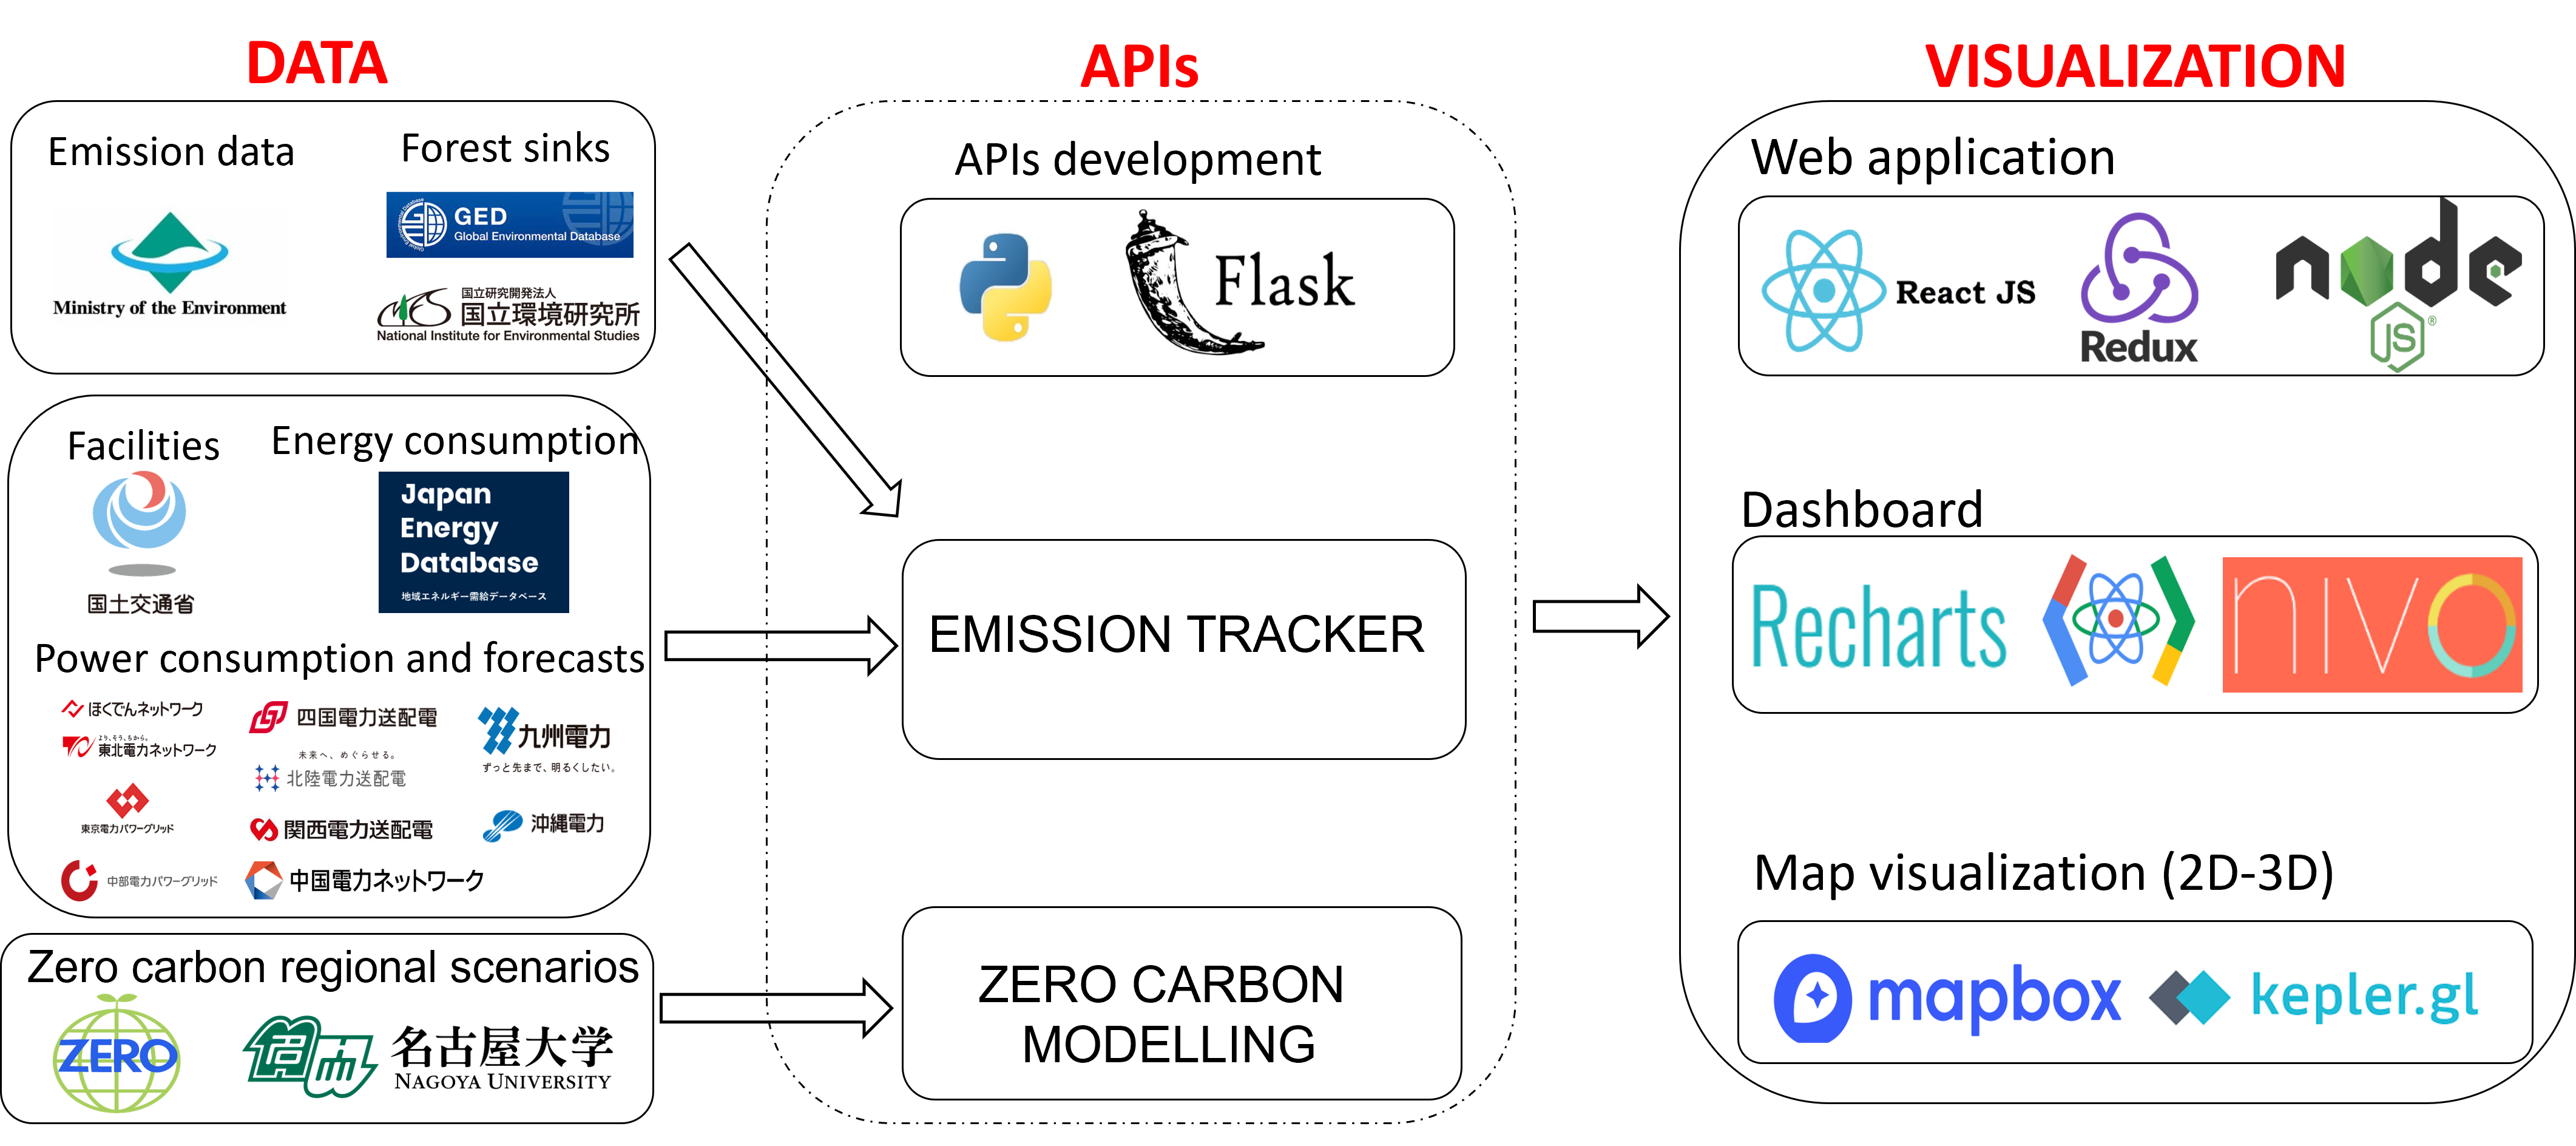
\includegraphics[width=\textwidth]{figs/chap7/platform_architecture.png}
  \caption[Platform architecture]{Platform Architecture and the technology used to develop the GIS platform}
  \label{fig:chap7_fig1}
\end{figure}

By leveraging cutting-edge GIS technology, this platform enables decision-makers to visualize and comprehend greenhouse gas (GHG) emissions data from various sectors. It facilitates the analysis and understanding of distinctive features, empowering informed policy decisions based on integrated information aimed at mitigating the impacts of climate change. \par
\subsection{Data collection}
Table 1 summarizes the details of the datasets introduced into the GIS platform, including the corresponding data sources, their respective purposes, and the display pages within the developed platform.\par

\begin{table}[!ht]
    \centering
    \caption{The dataset used for the GIS platform development}
    \begin{adjustbox}{width=\textwidth}
        \begin{tabular}{l l}
        \hline
            Dataset & Data source \\ \hline
            CO2 emissions by sector & \citep{env2022} \\ \hline
            Energy consumption statistics & \citep{Toshihiko} \\ \hline
            Power generation facility & \citep{nlftp} \\ \hline
            \multirow{10}{*}{Power consumption and forecasts} & \citep{hokkaido} \\
            ~ & \citep{tohoku} \\
            ~ & \citep{Tokyo} \\
            ~ & \citep{Chubu} \\
            ~ & \citep{Hokuriku} \\
            ~ & \citep{Kansai} \\
            ~ & \citep{Chugoku} \\
            ~ & \citep{Shikoku} \\
            ~ & \citep{Kyushu} \\
            ~ & \citep{Okinawa} \\ \hline
            Gross Primary Production & \multirow{3}{*}{\citep{ito2019disequilibrium}} \\
            Net Ecosystem Production & ~ \\
            Ecosystem respiration & ~ \\ \hline
            Zero carbon regional scenario & \citep{zerocarbon} \\
            \hline
        \end{tabular}
    \end{adjustbox}
    \label{tab:chap7_tab1}
\end{table}

\subsection{API development}
In developing the API to process these data, we utilized Flask, a micro web framework written in Python, and adhered to the JSON API specification for data format. The API of this system visualizes the dashboards for Emission Tracker and Zero Emission Modeling (Drawdown). JSON serves as the primary data format for the API, and all responses adhere to the specifications described in Table 2. The API is deployed on the cloud-based platform Heroku. \par


\begin{table}[!ht]
  \centering
  \caption{APIs specifications}
  \begin{adjustbox}{width=\textwidth}
      \begin{tabular}{lll}
        \hline
        End point & Parameters & Description \\ \hline
        GET /overall\_ems/country  & year: year of the emission data  & Emissions at national level \\ \hline
        \multirow{2}{*}{GET /overall\_ems/municipality}  & adm\_code: municipality code  & Emissions at municipality level in a specific year \\ 
        ~ & year: year of the emission data  & ~ \\ \hline
        GET /overall\_ems/municipality\_ts  & adm\_code: municipality code  & Time-series emissions at municipality level.  \\ \hline
        GET /overall\_ems/sector  & sector\_type: sector type & Emissions categorized by sectors.  \\ \hline
        GET /ee\_stats/5mins  & None & Near real time power usage, forecast \\ \hline
        GET /ee\_stats/energy\_consumption  & adm\_code: municipality code  & Energy consumption at municipality level.  \\ \hline
        GET /forest\_sink/municipality  & adm\_code: municipality code  & Forest variable at municipality level.  \\ \hline
        \multirow{2}{*}{GET /industry/annual\_ems}  & adm\_code: municipality code & Industrial emission at municipality level \\ 
        ~ & year: year of the emission data & ~ \\ \hline
        GET /zero\_ems/municipality & adm\_code: municipality code & Roadmap to reduce GHG at municipality level \\ \hline
    \end{tabular}
  \end{adjustbox}
  \label{tab:chap7_tab2}
\end{table}

\subsection{Web application}

In a web application, there are two main functions: (1) Understanding the Reality of CO2 Emissions – Emission Tracker and (2) Modeling a Carbon-Zero Scenario (Drawdown). First, in the CO2 Emission Tracker, it provides an overview of emissions and forest absorption at the local government level. Additionally, it offers data on energy consumption, such as electricity, to aid in understanding the current situation. Specifically, the CO2 Emission Tracker consists of five tabs with the following functions: an overview of emissions, forest absorption, energy consumption, electricity statistics, and emissions by industrial sector (specific establishments). In (2) Drawdown Modeling, it provides simulation results outlining a roadmap to maximize emission reduction by 2050. To build an interactive GIS dashboard, the platform development utilized the following technologies: \par

\begin{figure}[p]
  \centering
  \begin{subfigure}{.5\textwidth}
      \centering
      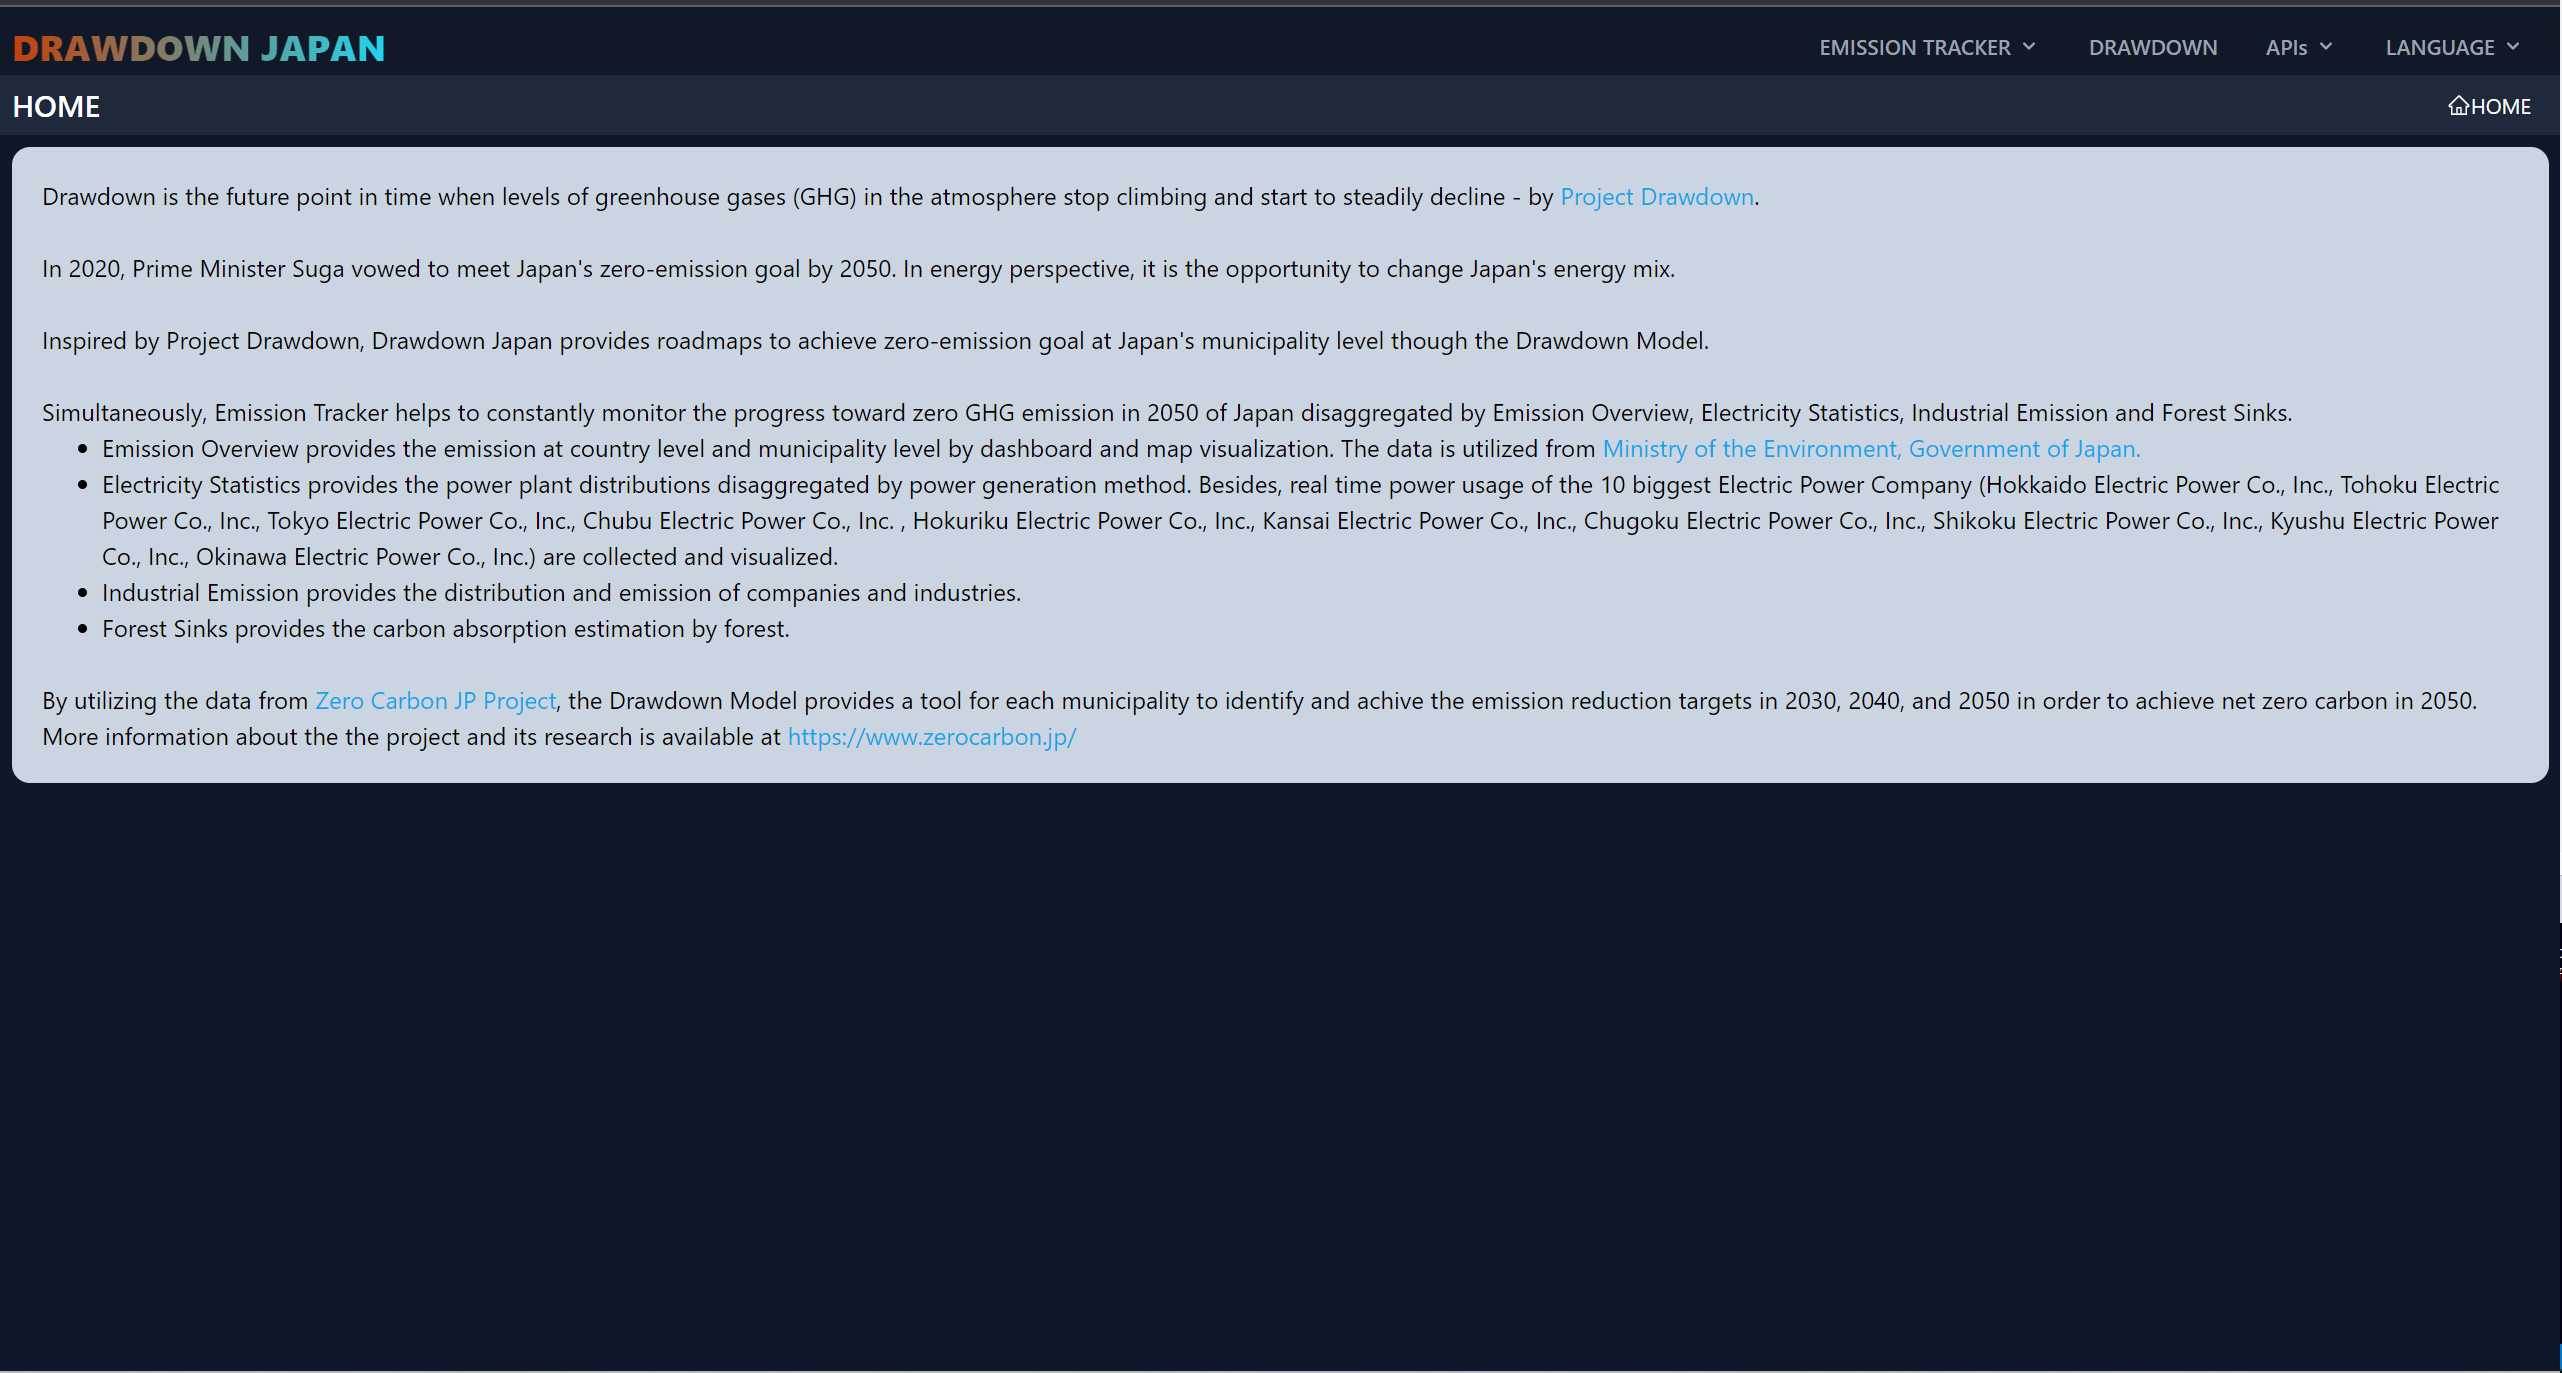
\includegraphics[width=.9\textwidth]{figs/chap7/home.png}
      \caption{Forest map in Ena City, Japan}
      % \label{fig:chap7_fig2a}
  \end{subfigure}%
  \begin{subfigure}{.5\textwidth}
      \centering
      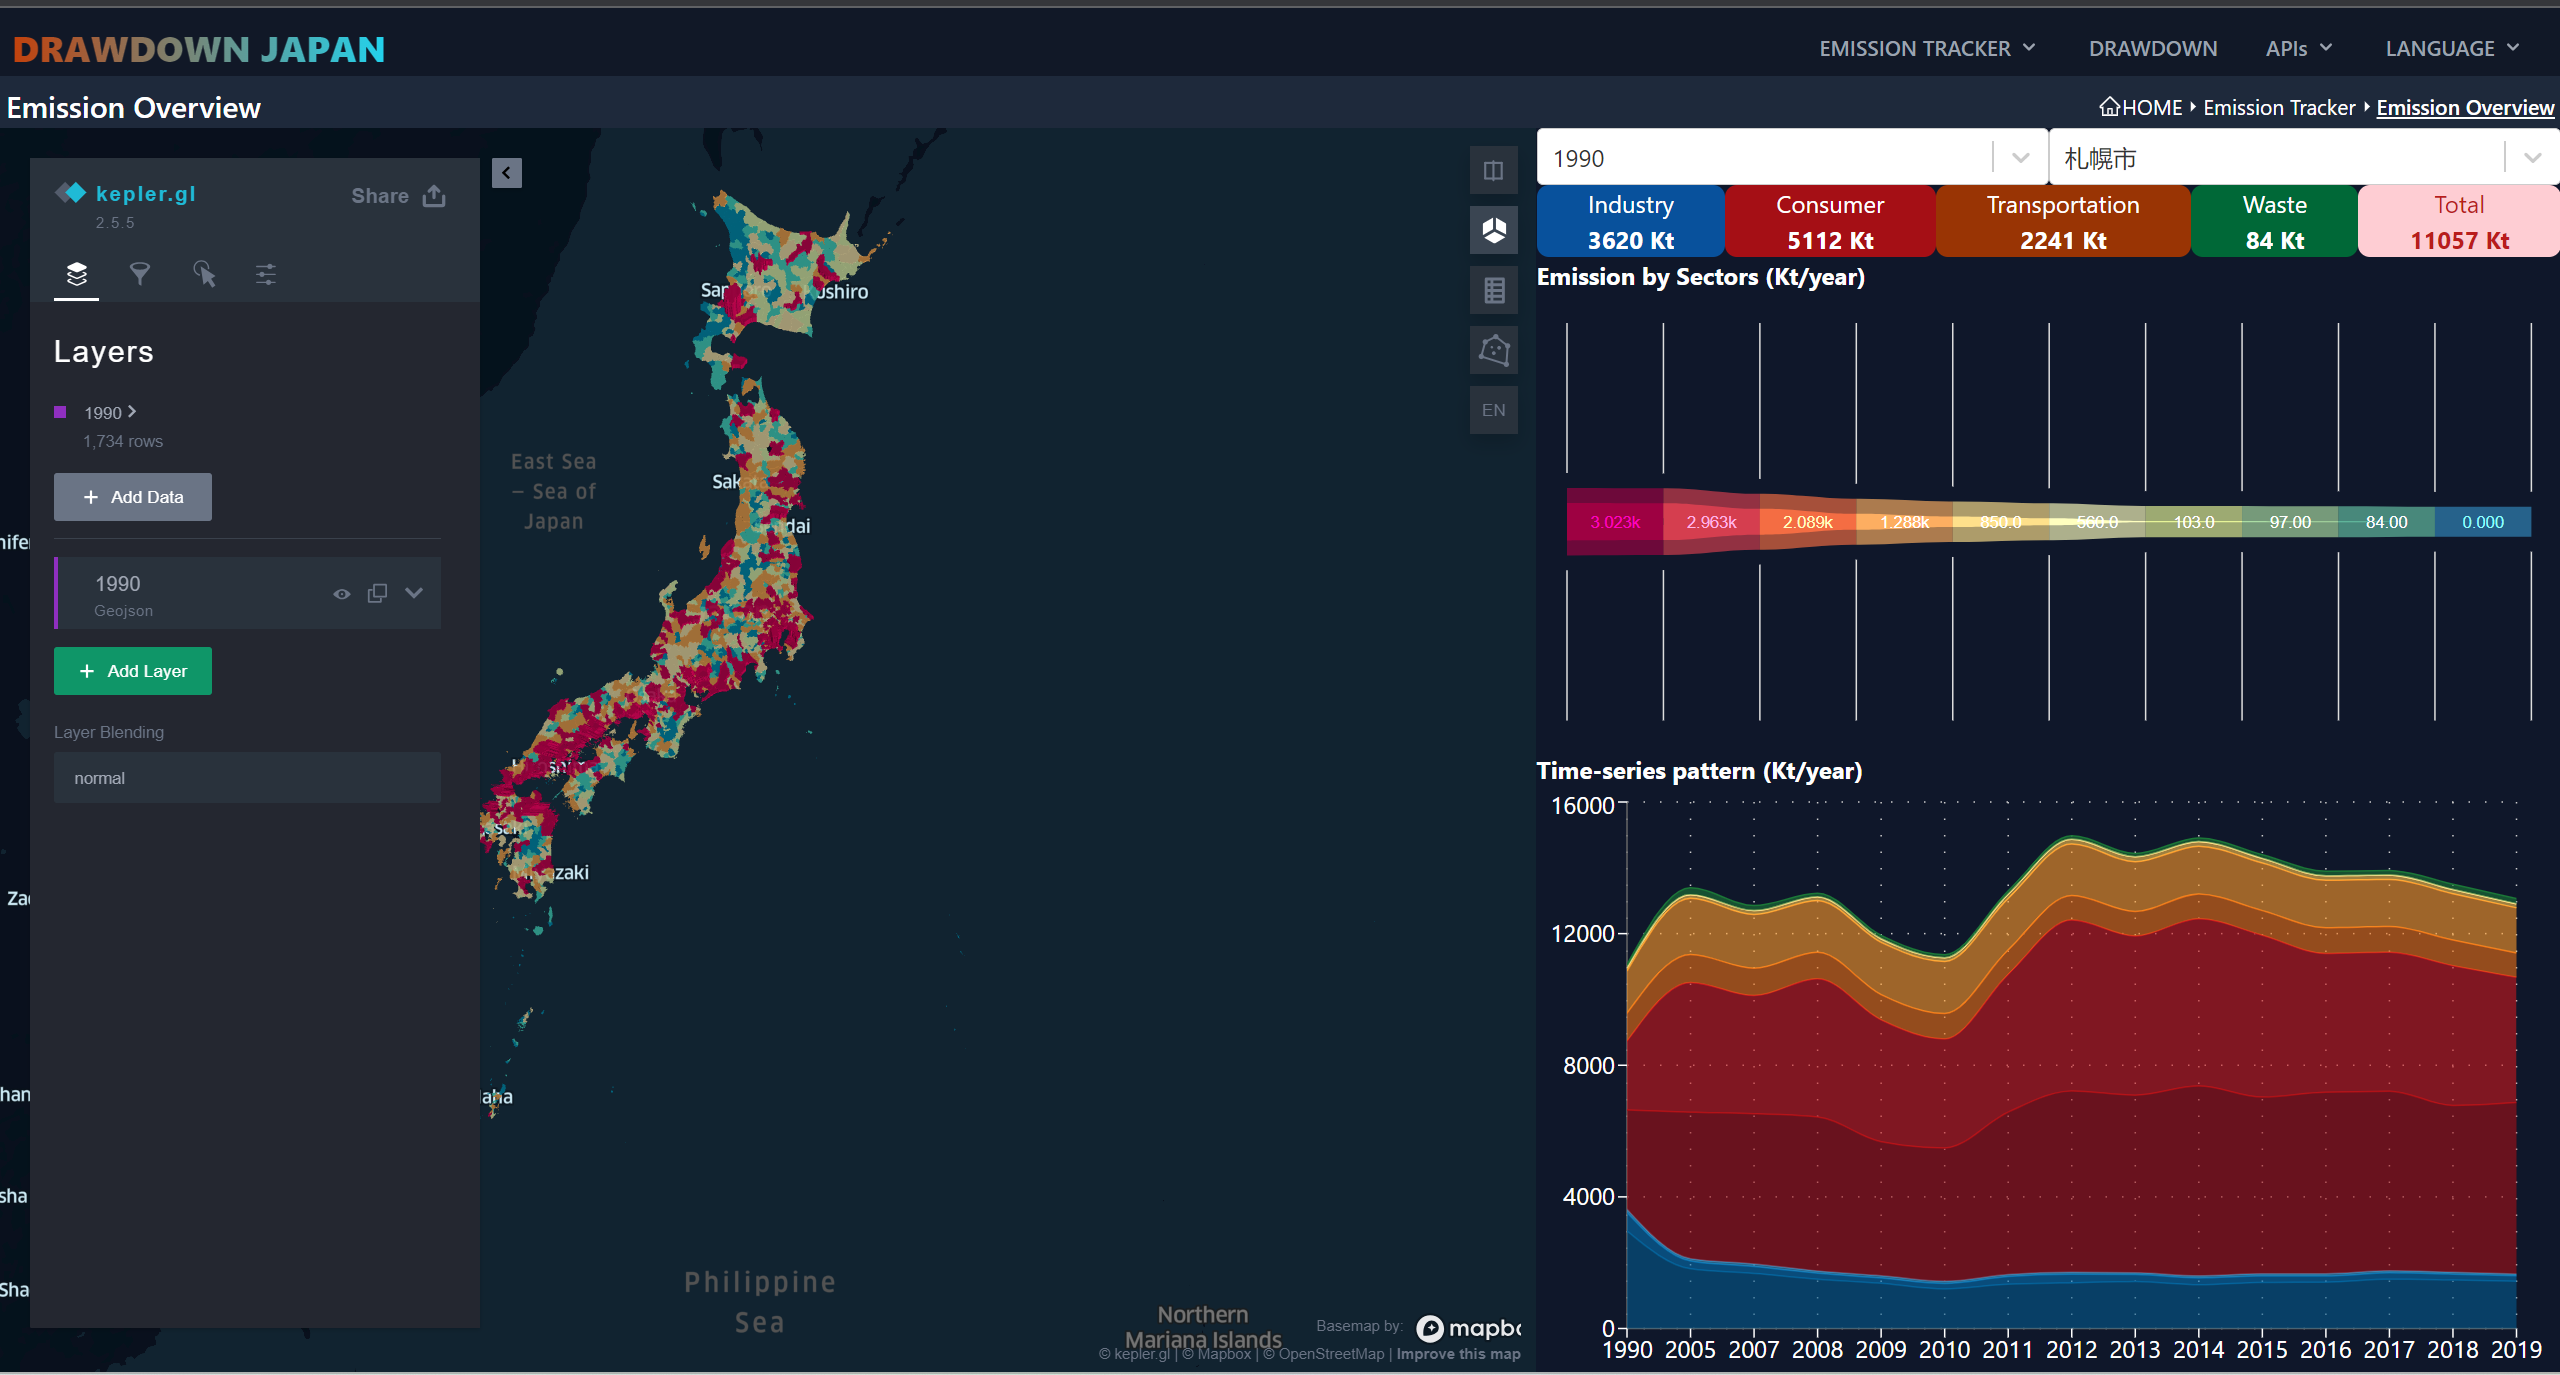
\includegraphics[width=.9\textwidth]{figs/chap7/ems_overview.png}
      \caption{Map overlays}
      % \label{fig:chap7_fig2b}
  \end{subfigure}

  \begin{subfigure}{.5\textwidth}
      \centering
      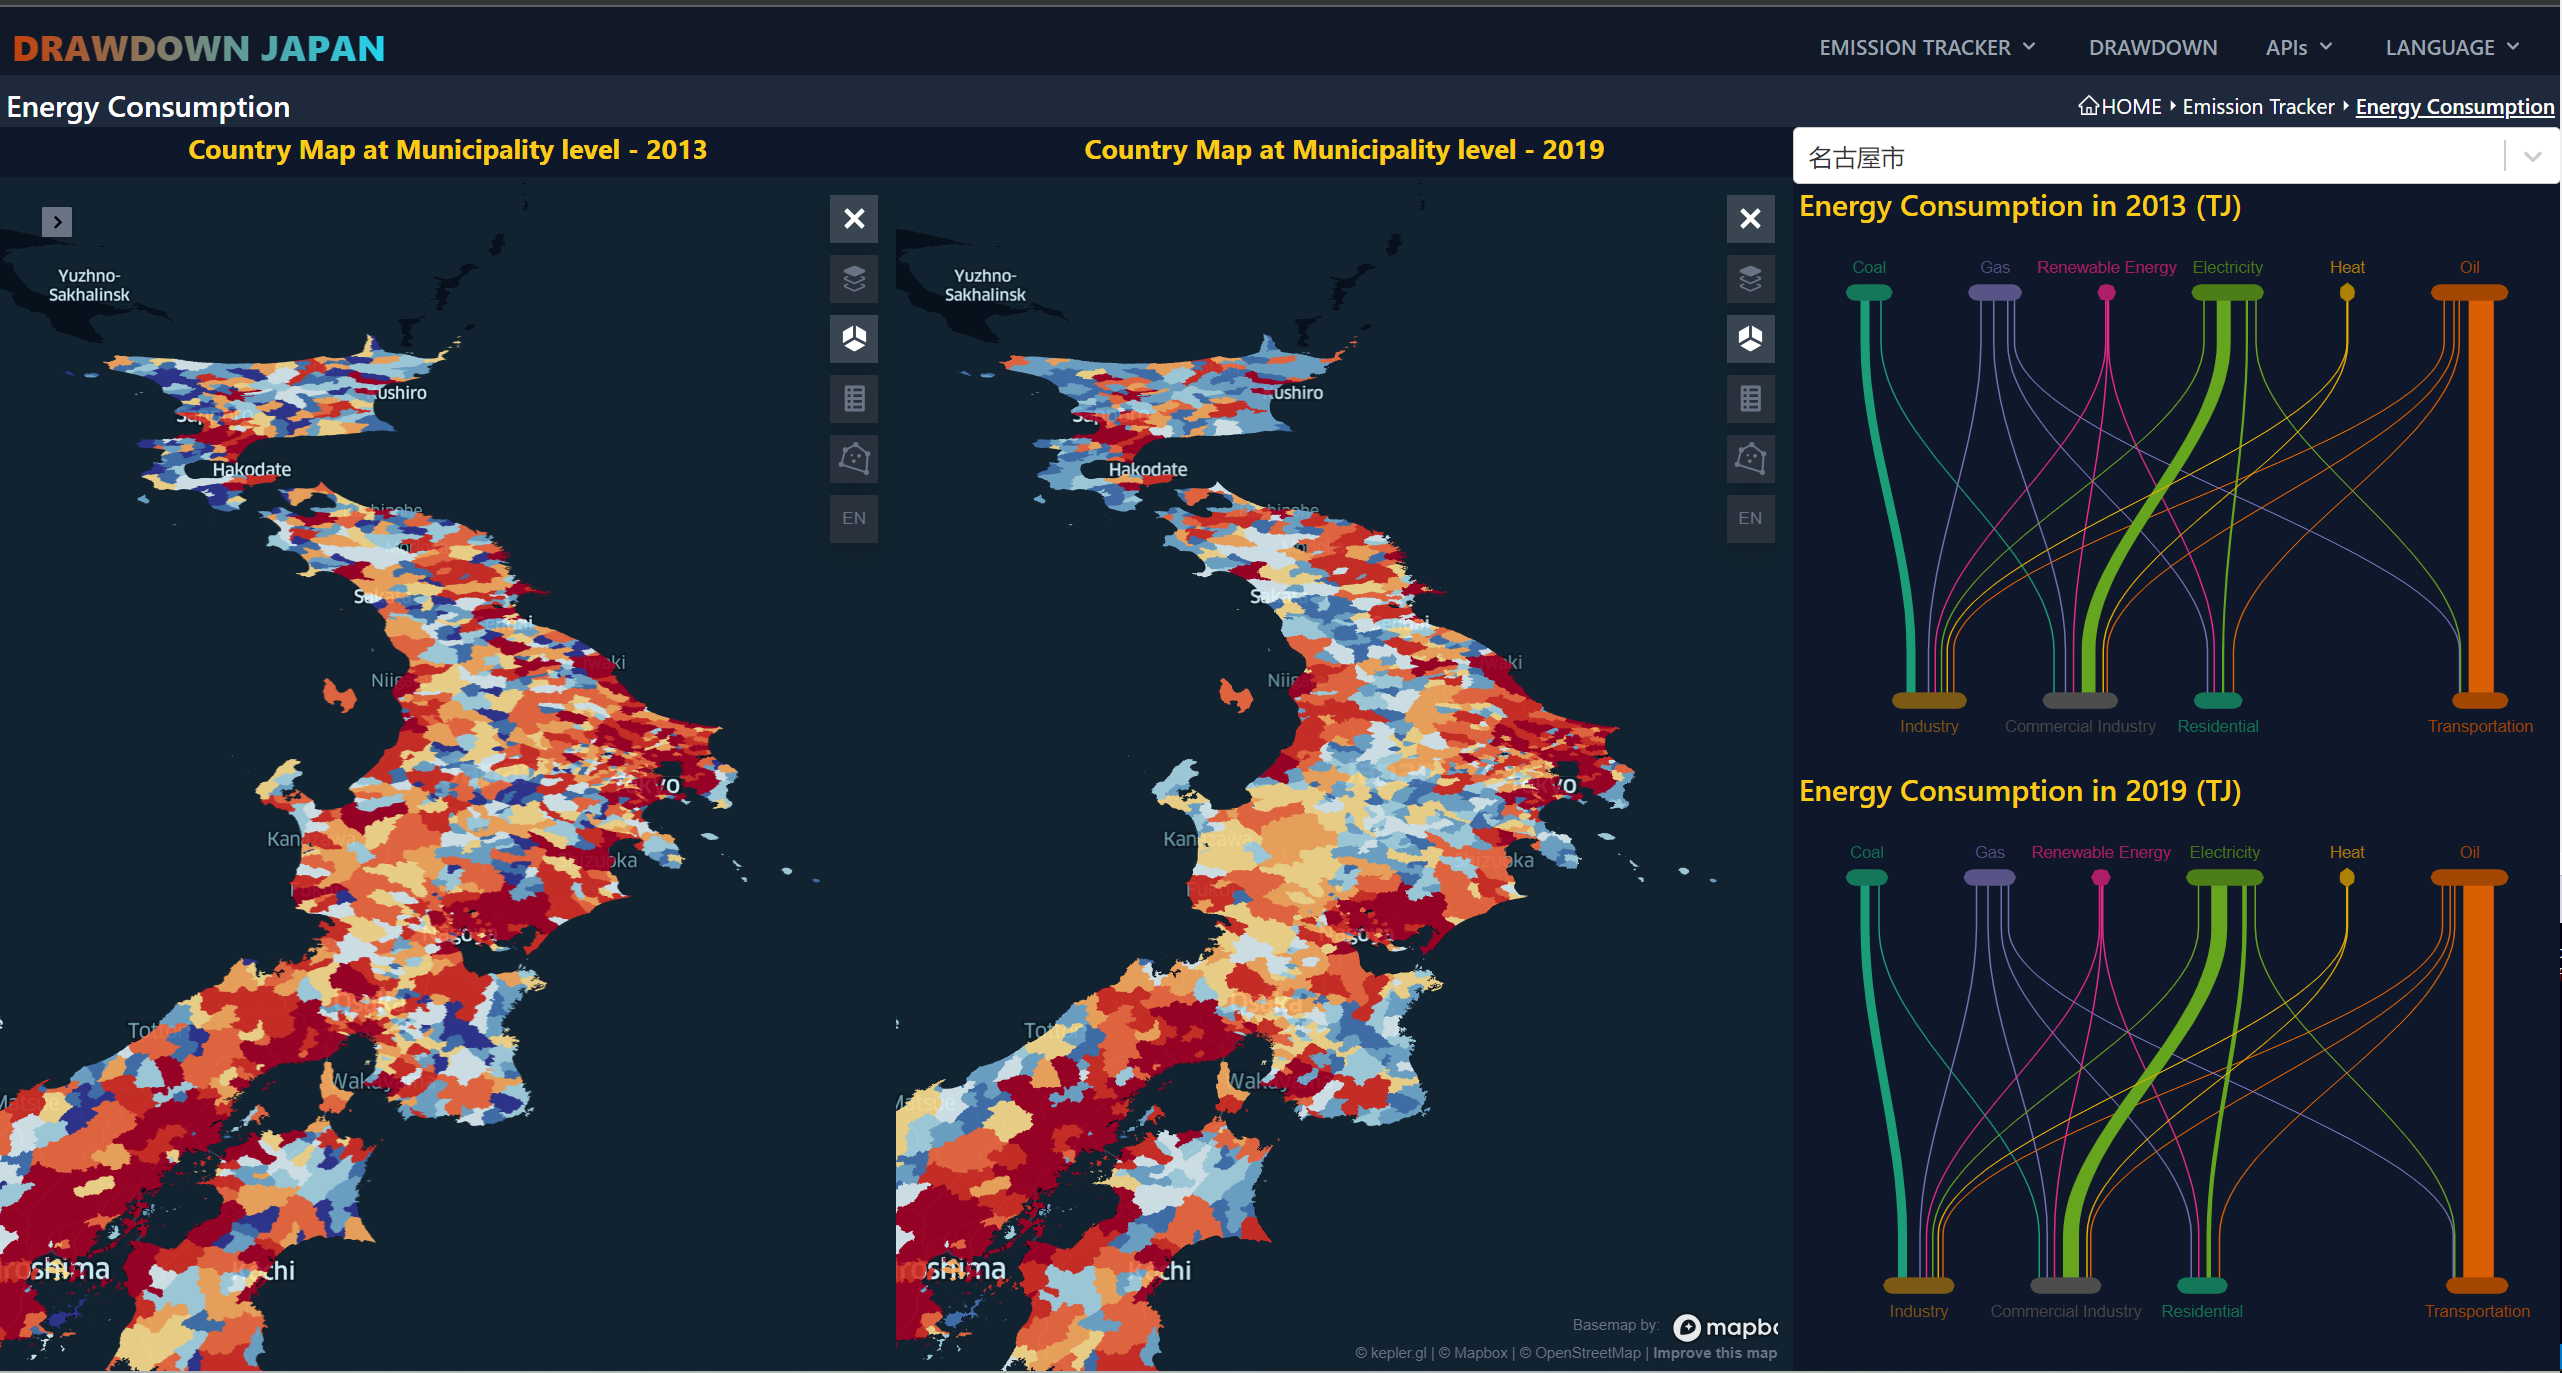
\includegraphics[width=.9\textwidth]{figs/chap7/ems_consumption.png}
      \caption{Forest map in Ena City, Japan}
      % \label{fig:chap7_fig2a}
  \end{subfigure}%
  \begin{subfigure}{.5\textwidth}
      \centering
      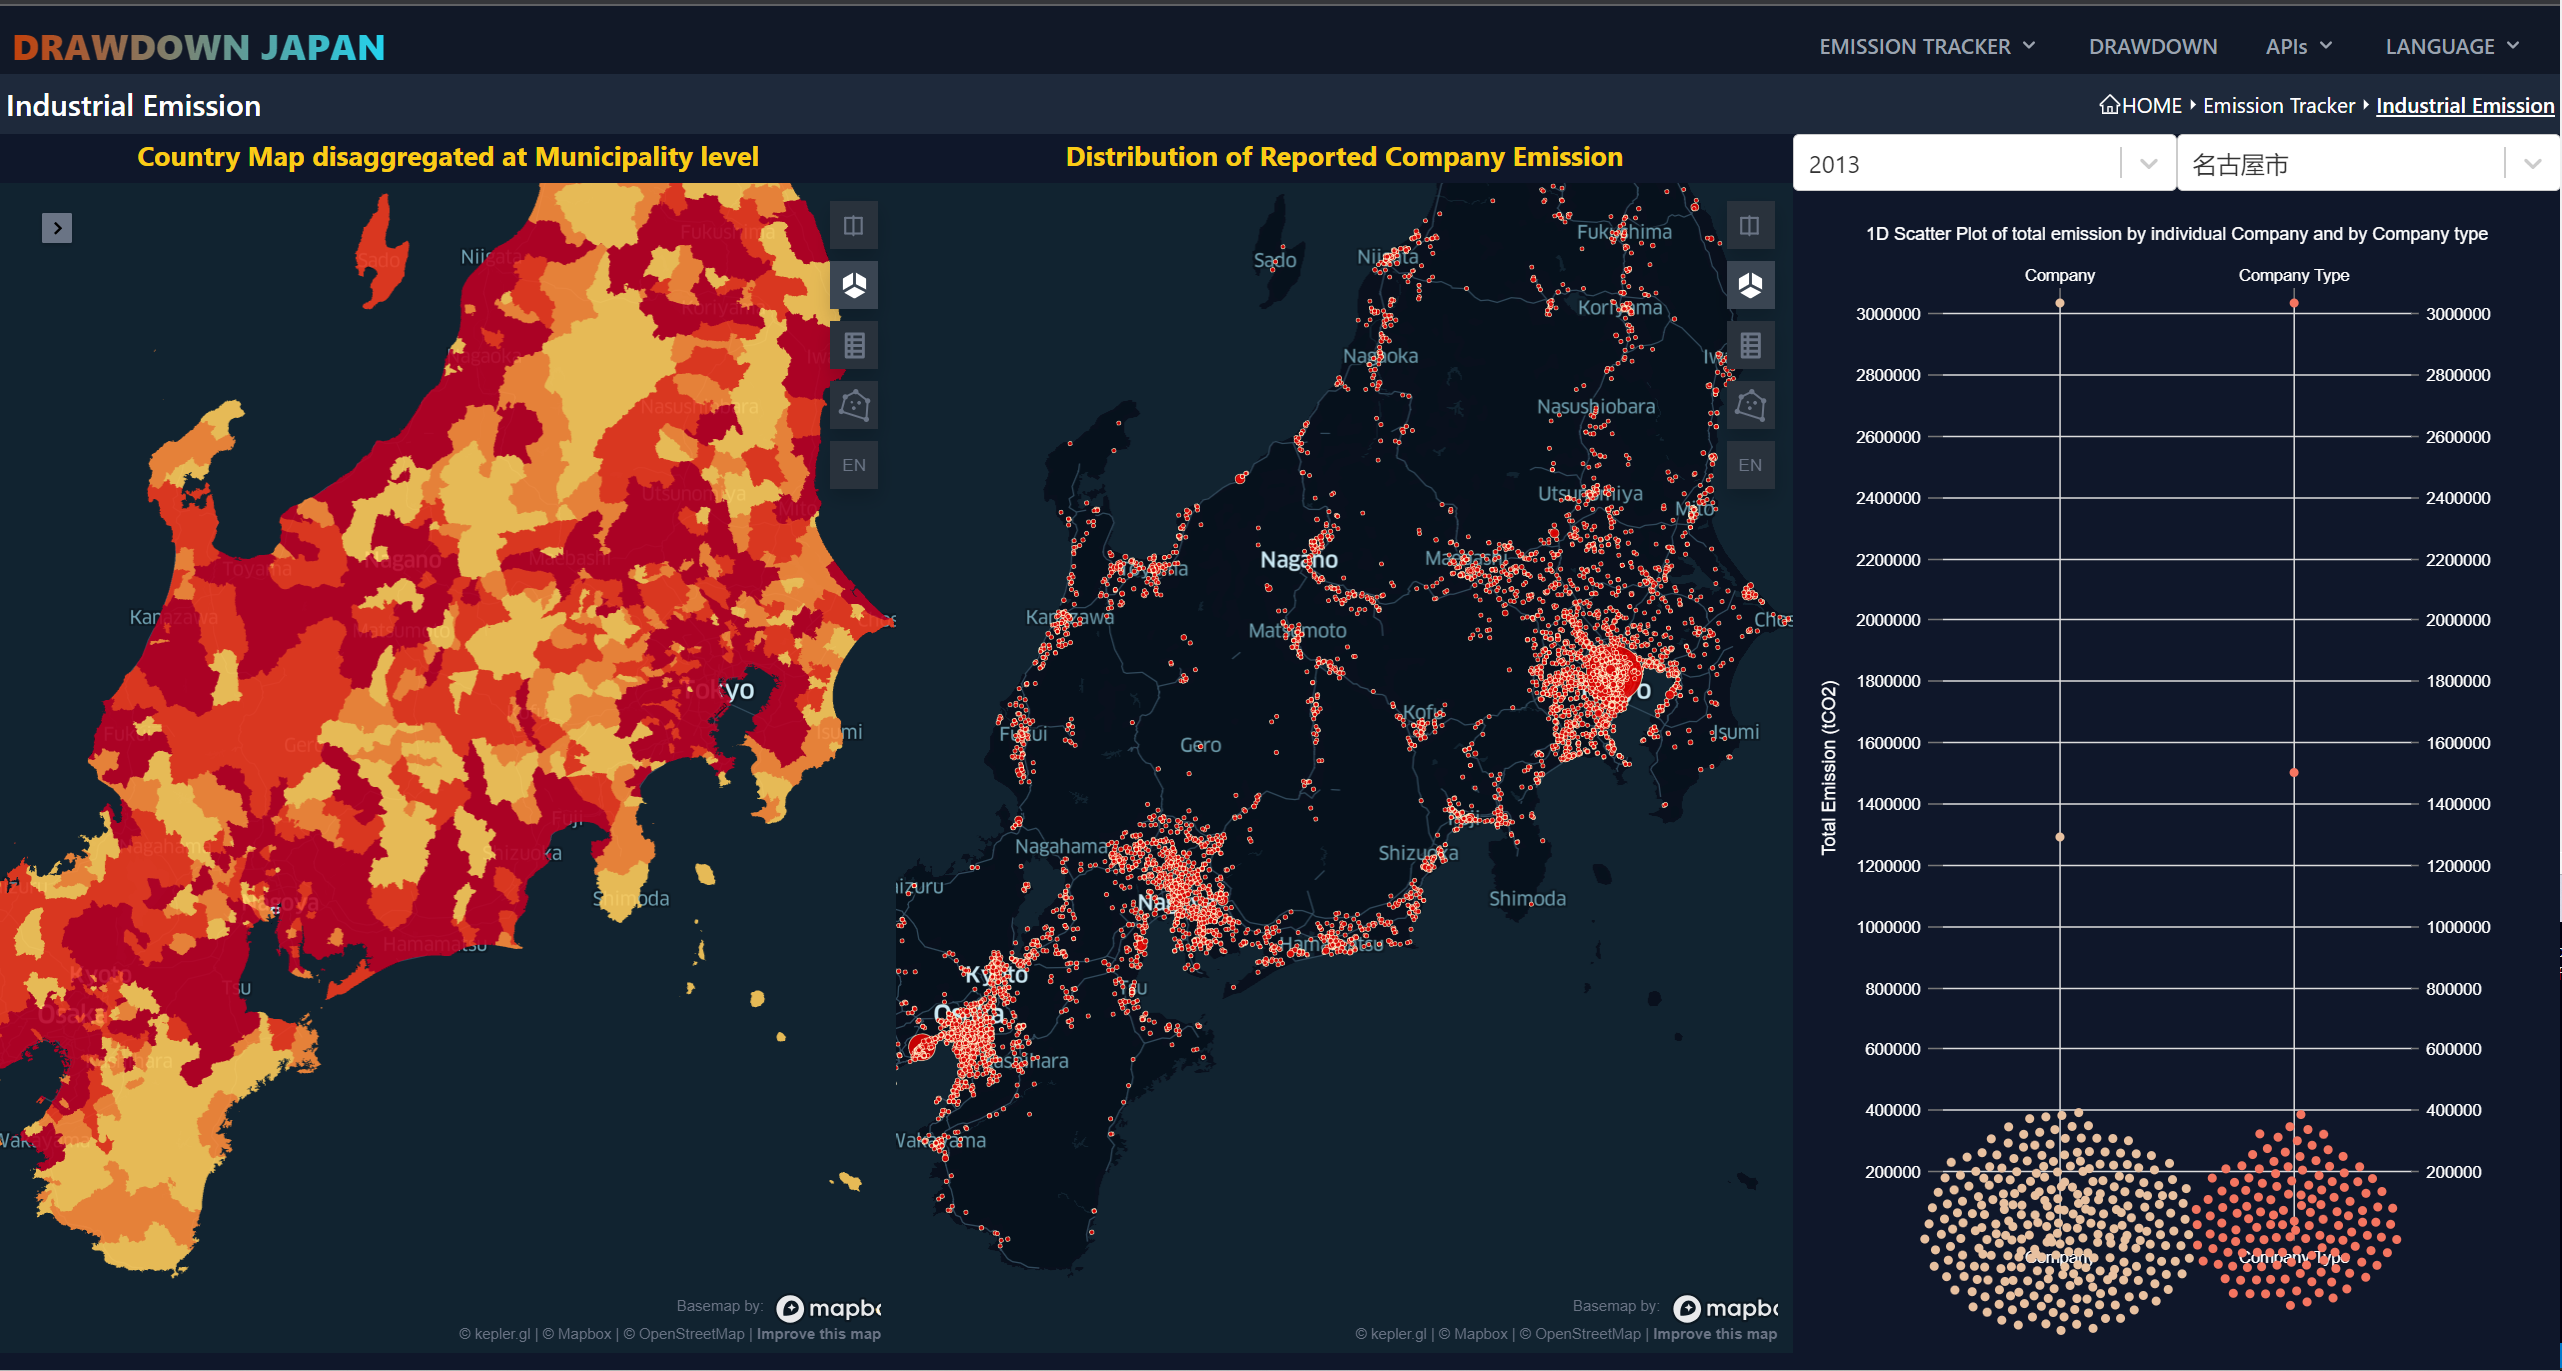
\includegraphics[width=.9\textwidth]{figs/chap7/industrial_ems.png}
      \caption{Map overlays}
      % \label{fig:chap7_fig2b}
  \end{subfigure}

  \begin{subfigure}{.5\textwidth}
    \centering
    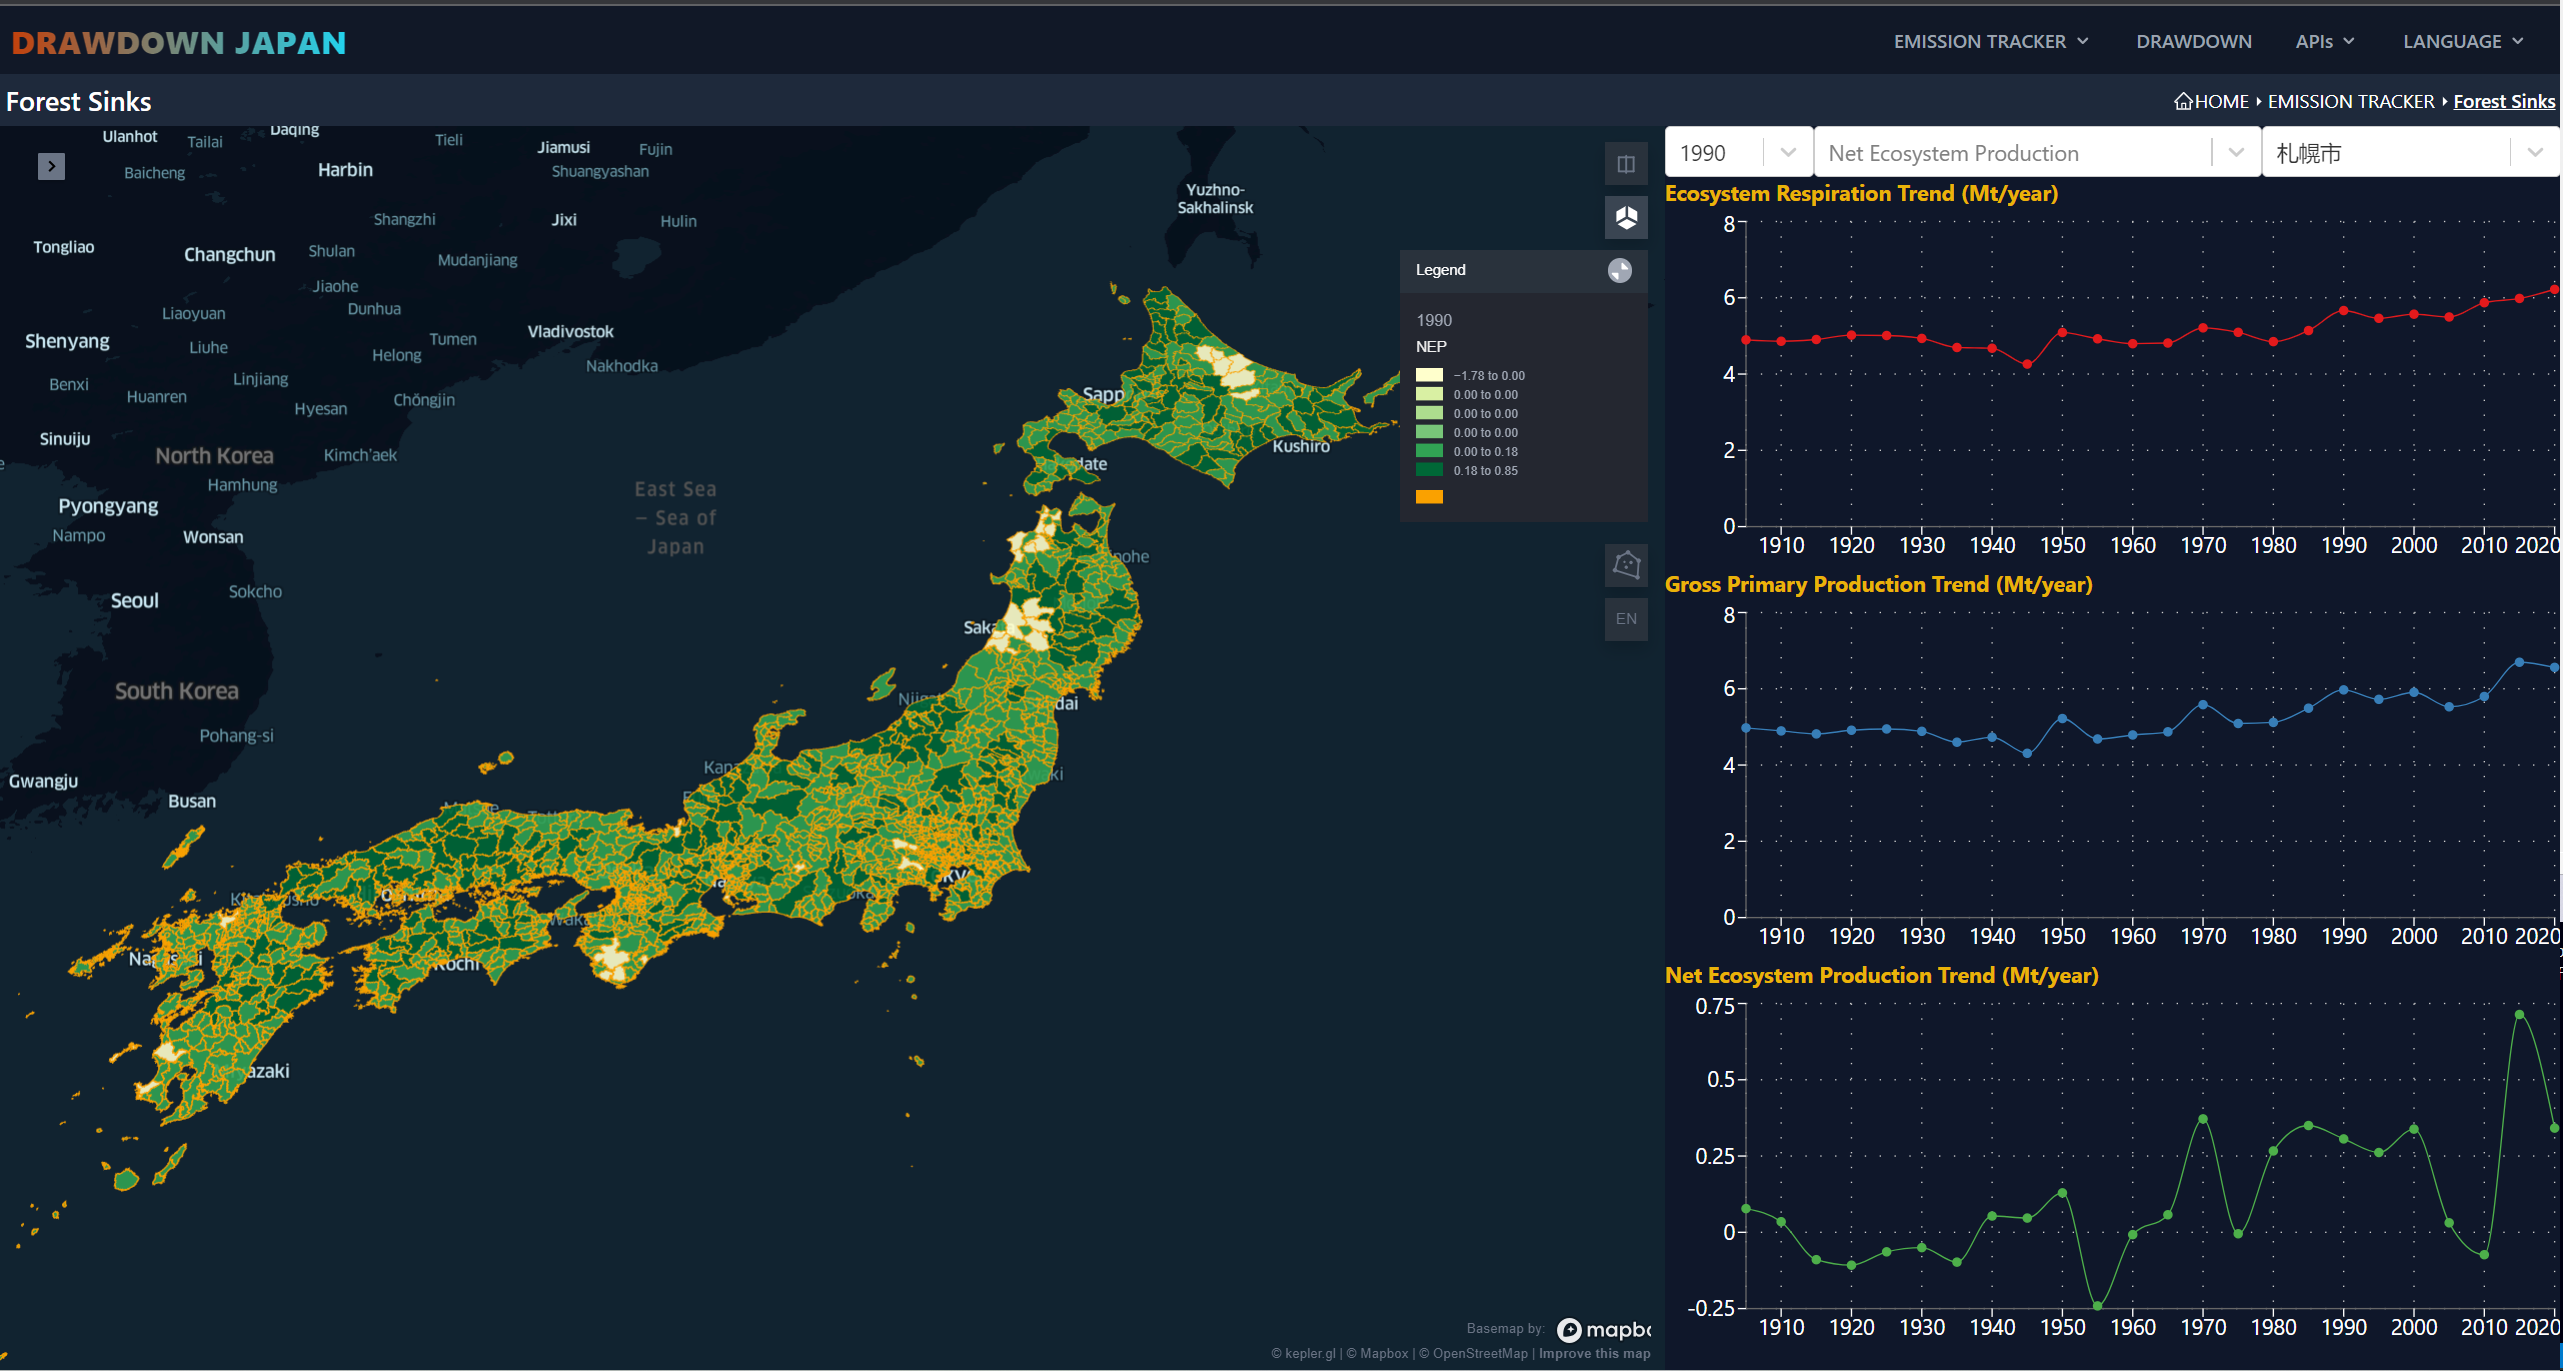
\includegraphics[width=.9\textwidth]{figs/chap7/ems_forest.png}
      \caption{Forest map in Ena City, Japan}
      % \label{fig:chap7_fig2a}
  \end{subfigure}%
  \begin{subfigure}{.5\textwidth}
      \centering
      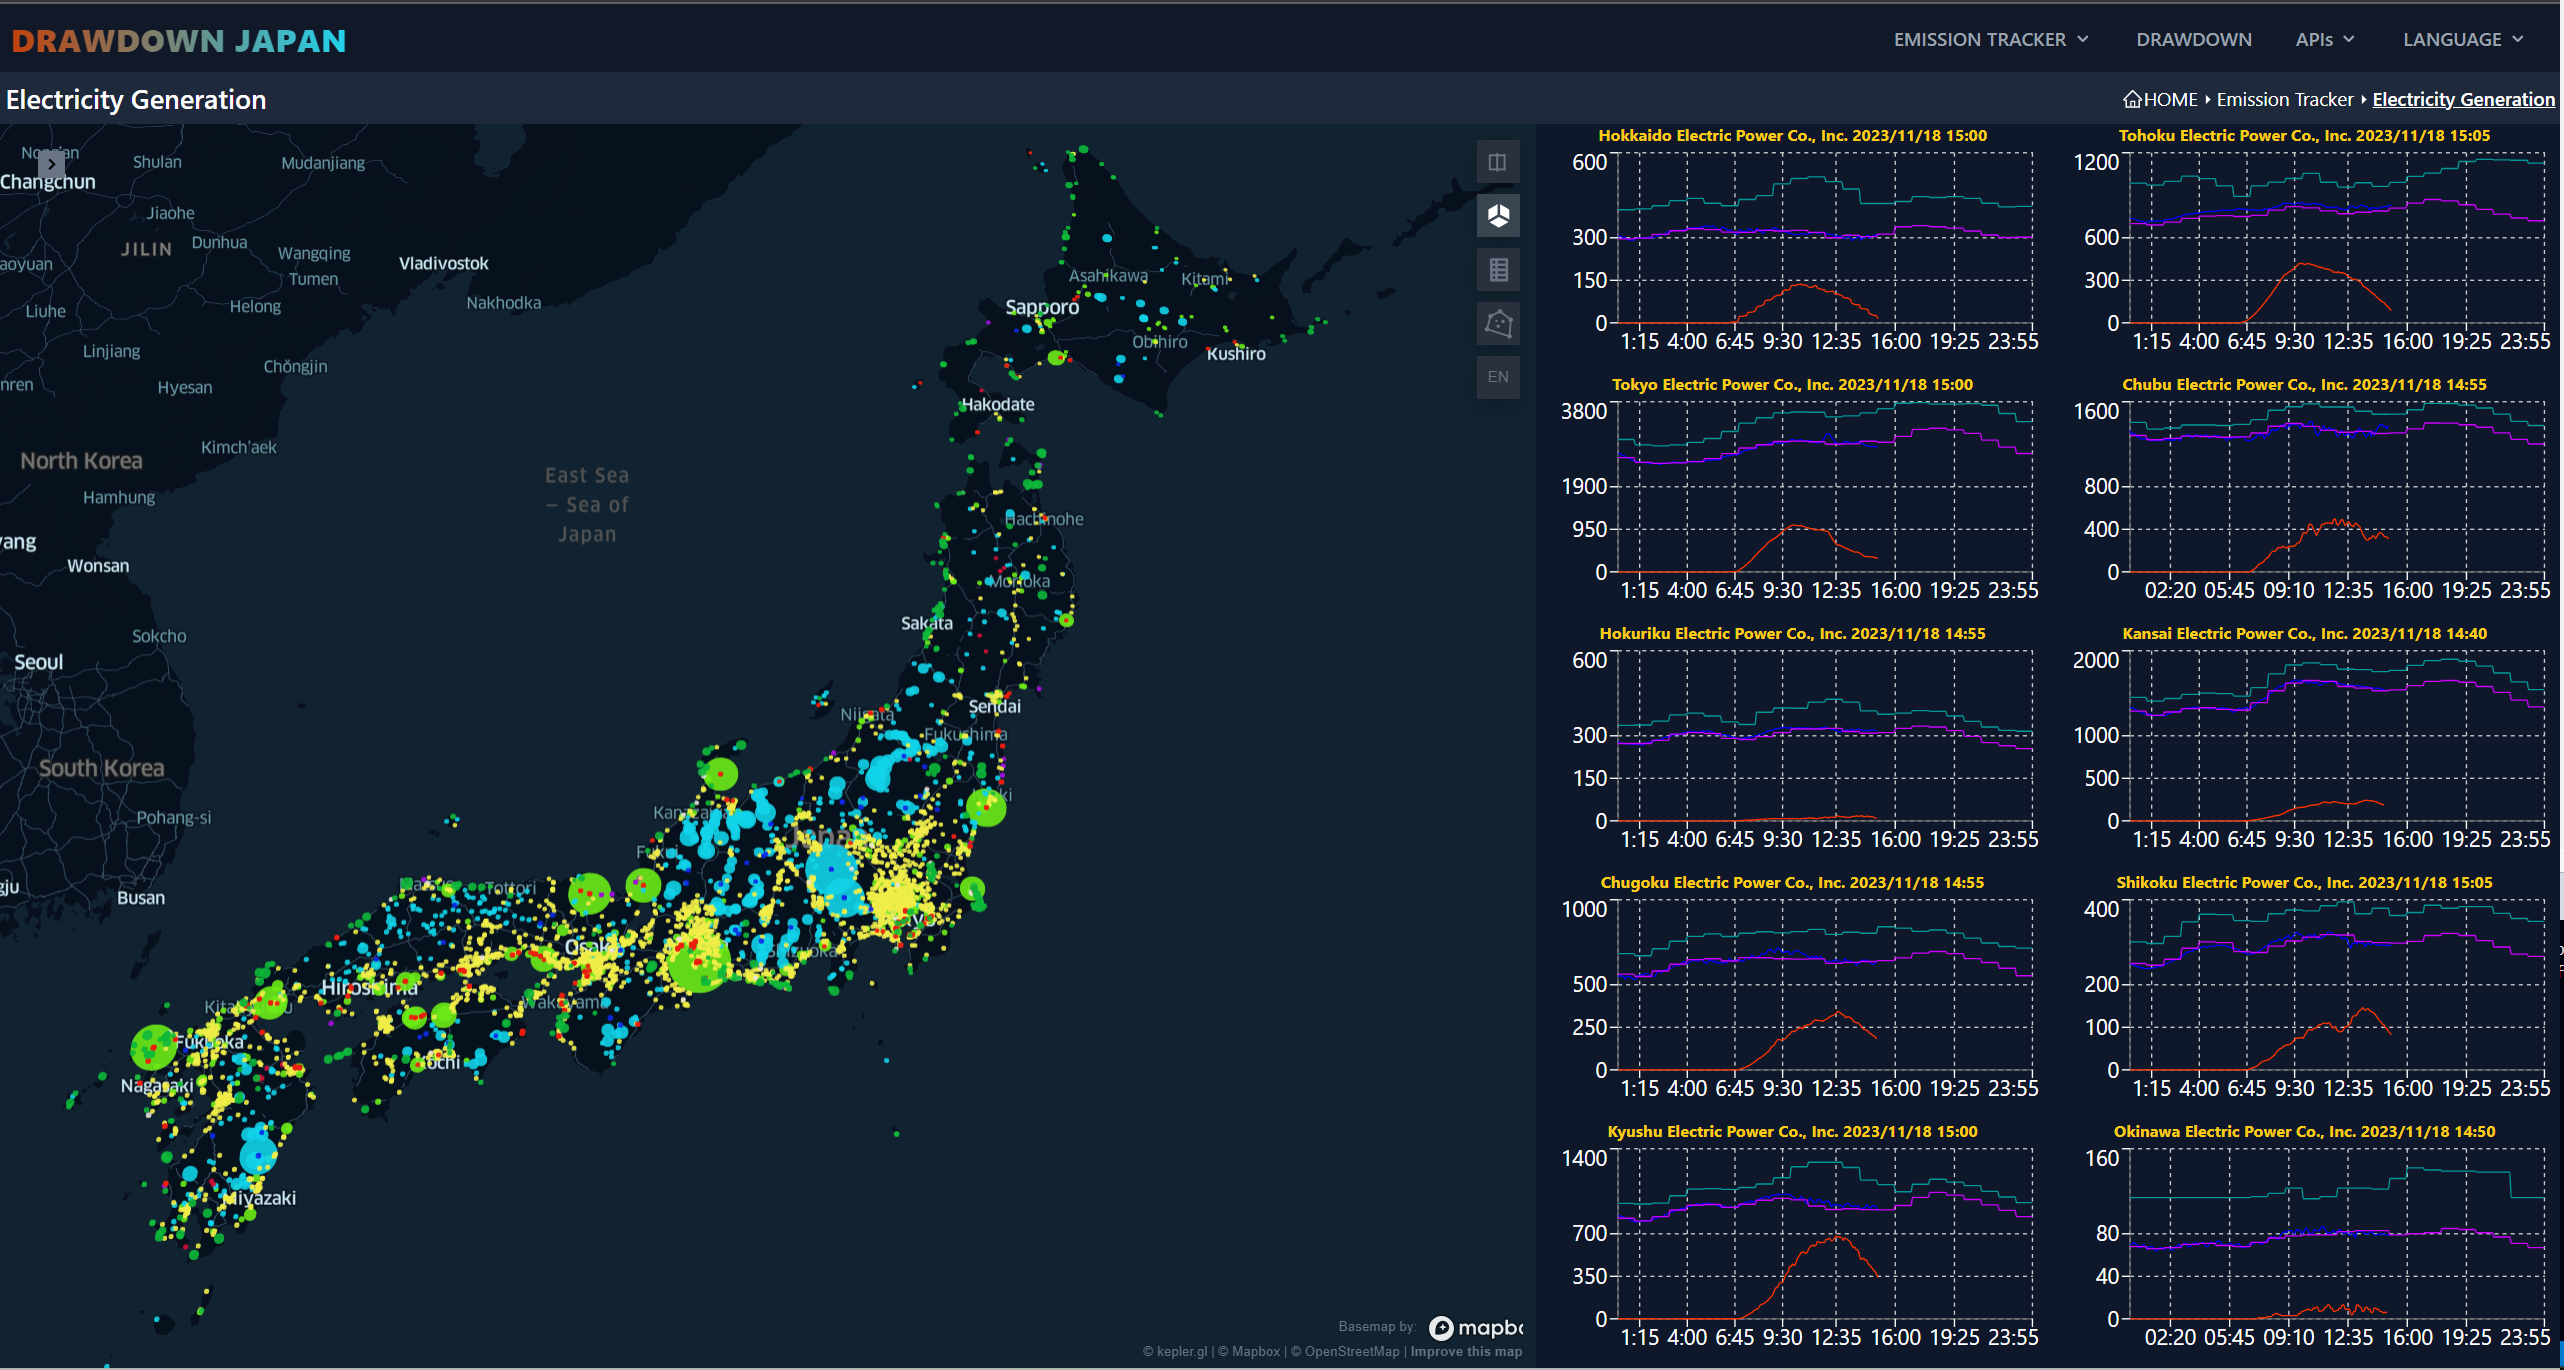
\includegraphics[width=.9\textwidth]{figs/chap7/ems_electric.png}
      \caption{Map overlays}
      % \label{fig:chap7_fig2b}
  \end{subfigure}
  \caption[Inferred forest map in Ena City]{Inferred forest map in Ena City, Japan \textminus 2018 (OA \textminus 94.5\%)}
  \label{fig:chap7_fig2}
\end{figure}


\begin{figure}[tbh!]
  \centering
  \begin{subfigure}{.5\textwidth}
      \centering
      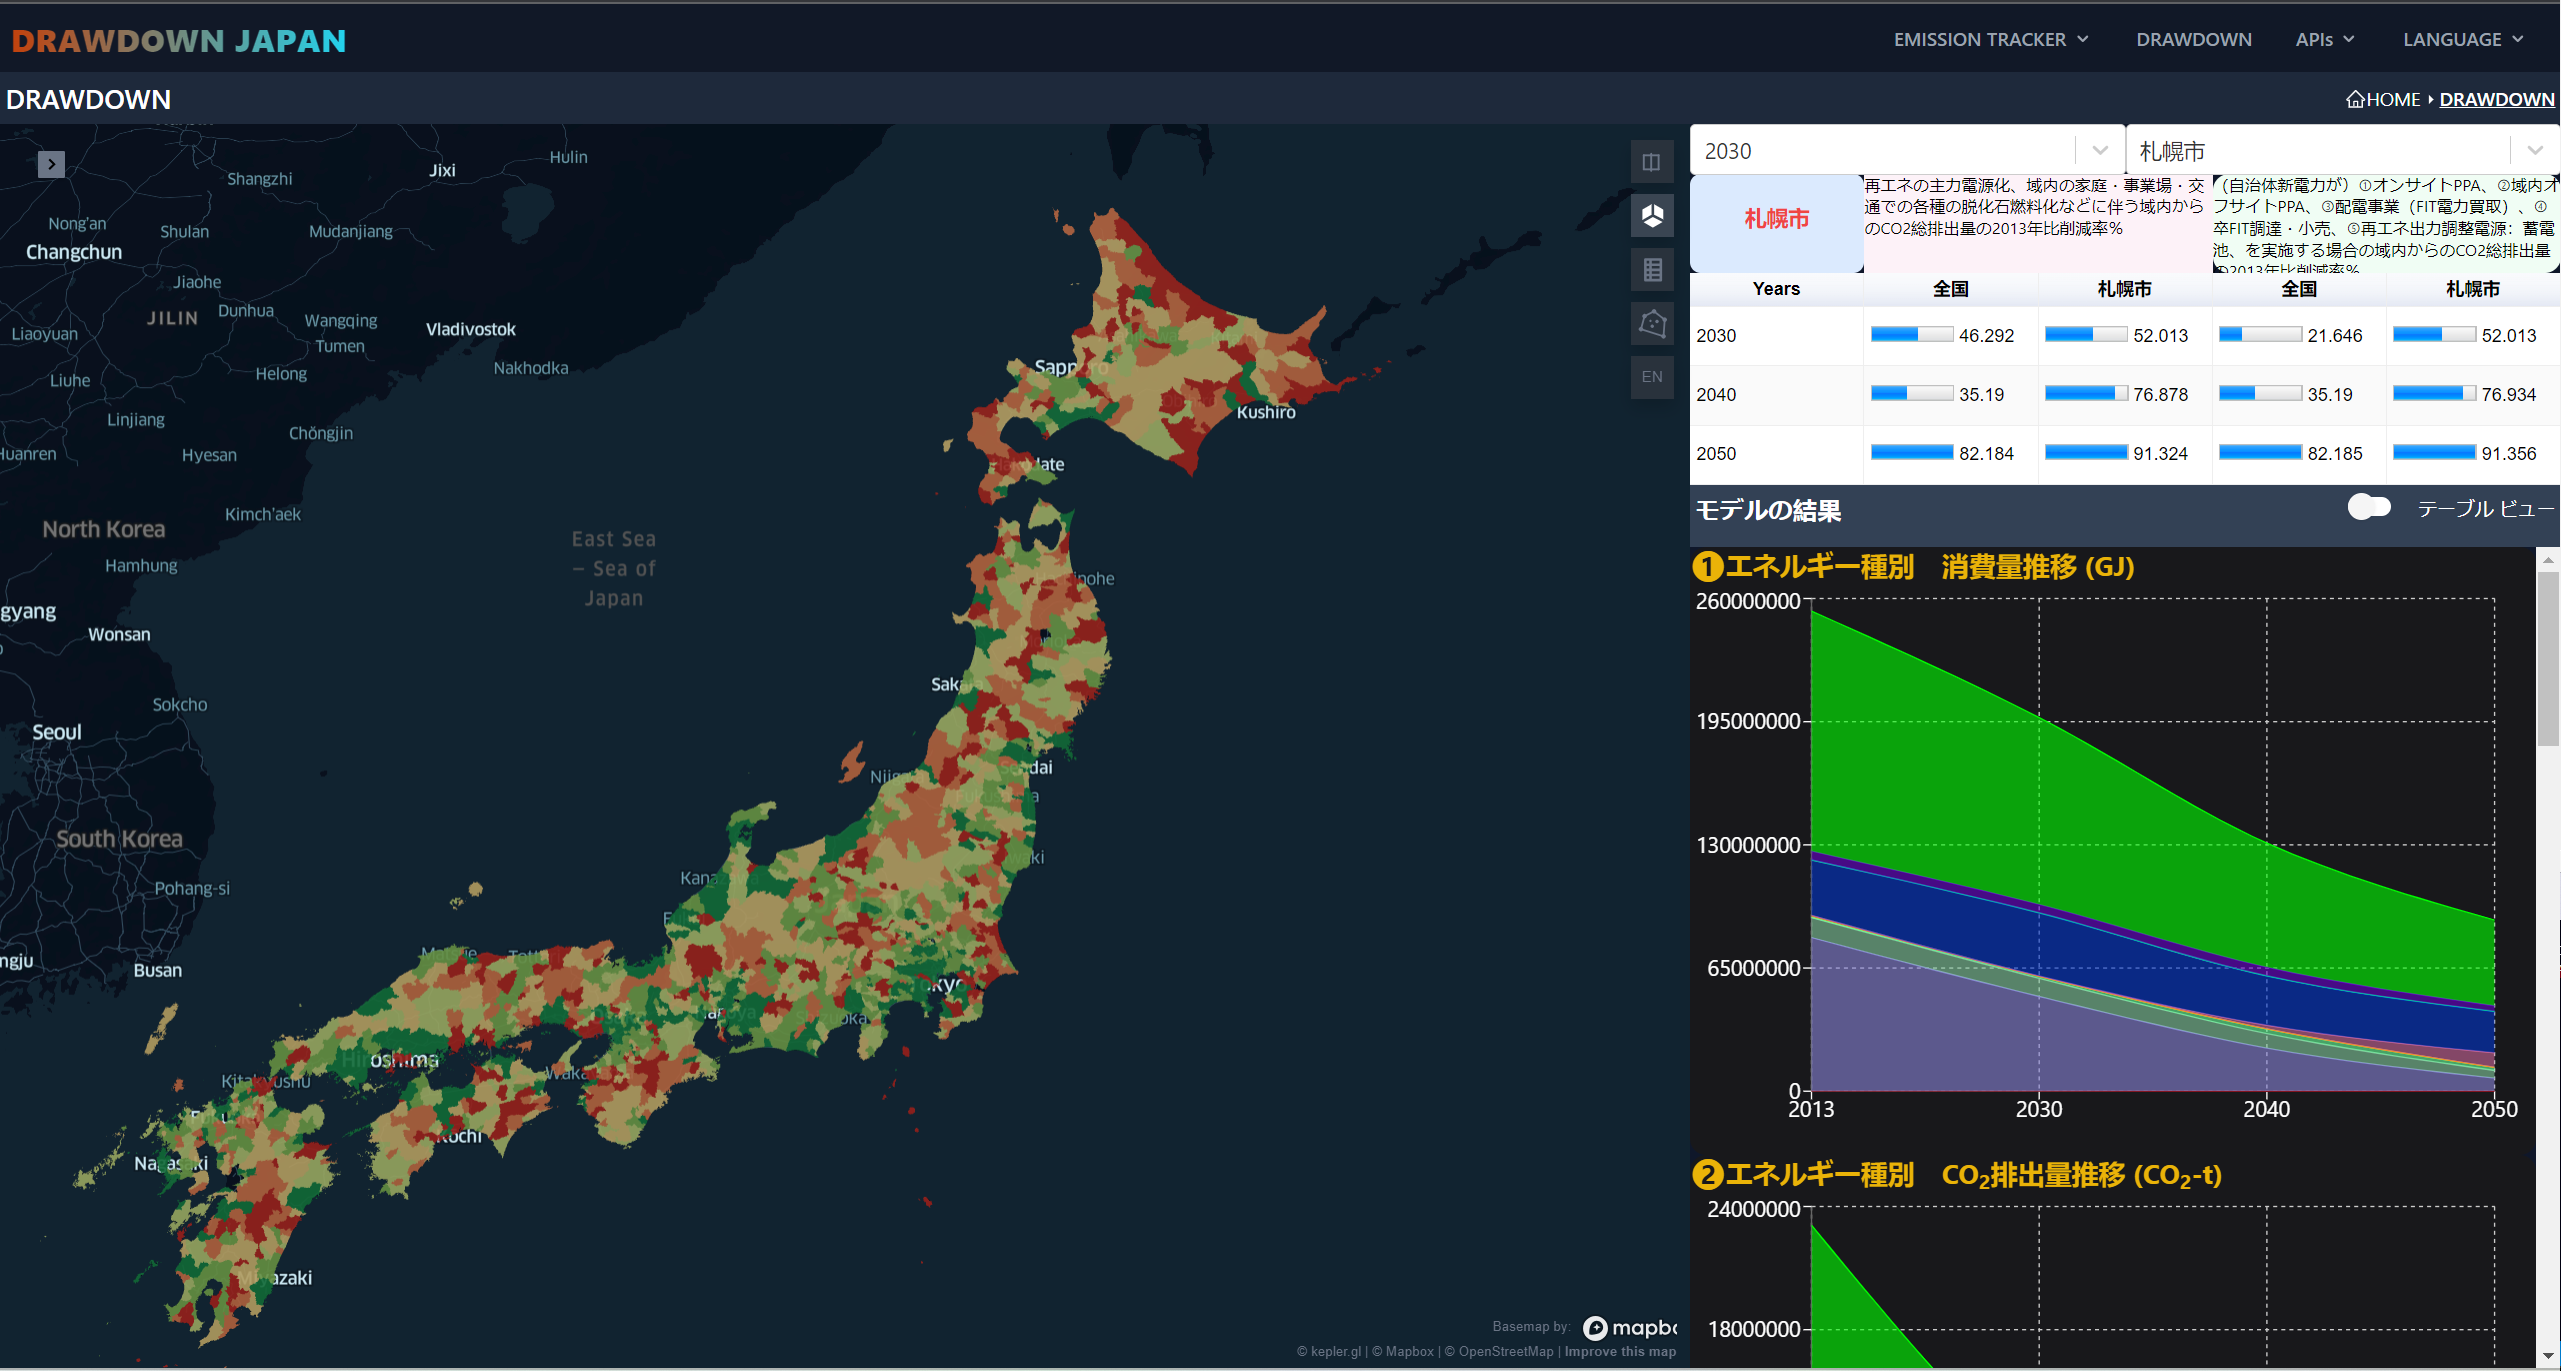
\includegraphics[width=.9\textwidth]{figs/chap7/drawdown1.png}
      \caption{Forest map in Ena City, Japan}
      % \label{fig:chap7_fig2a}
  \end{subfigure}%
  \begin{subfigure}{.5\textwidth}
      \centering
      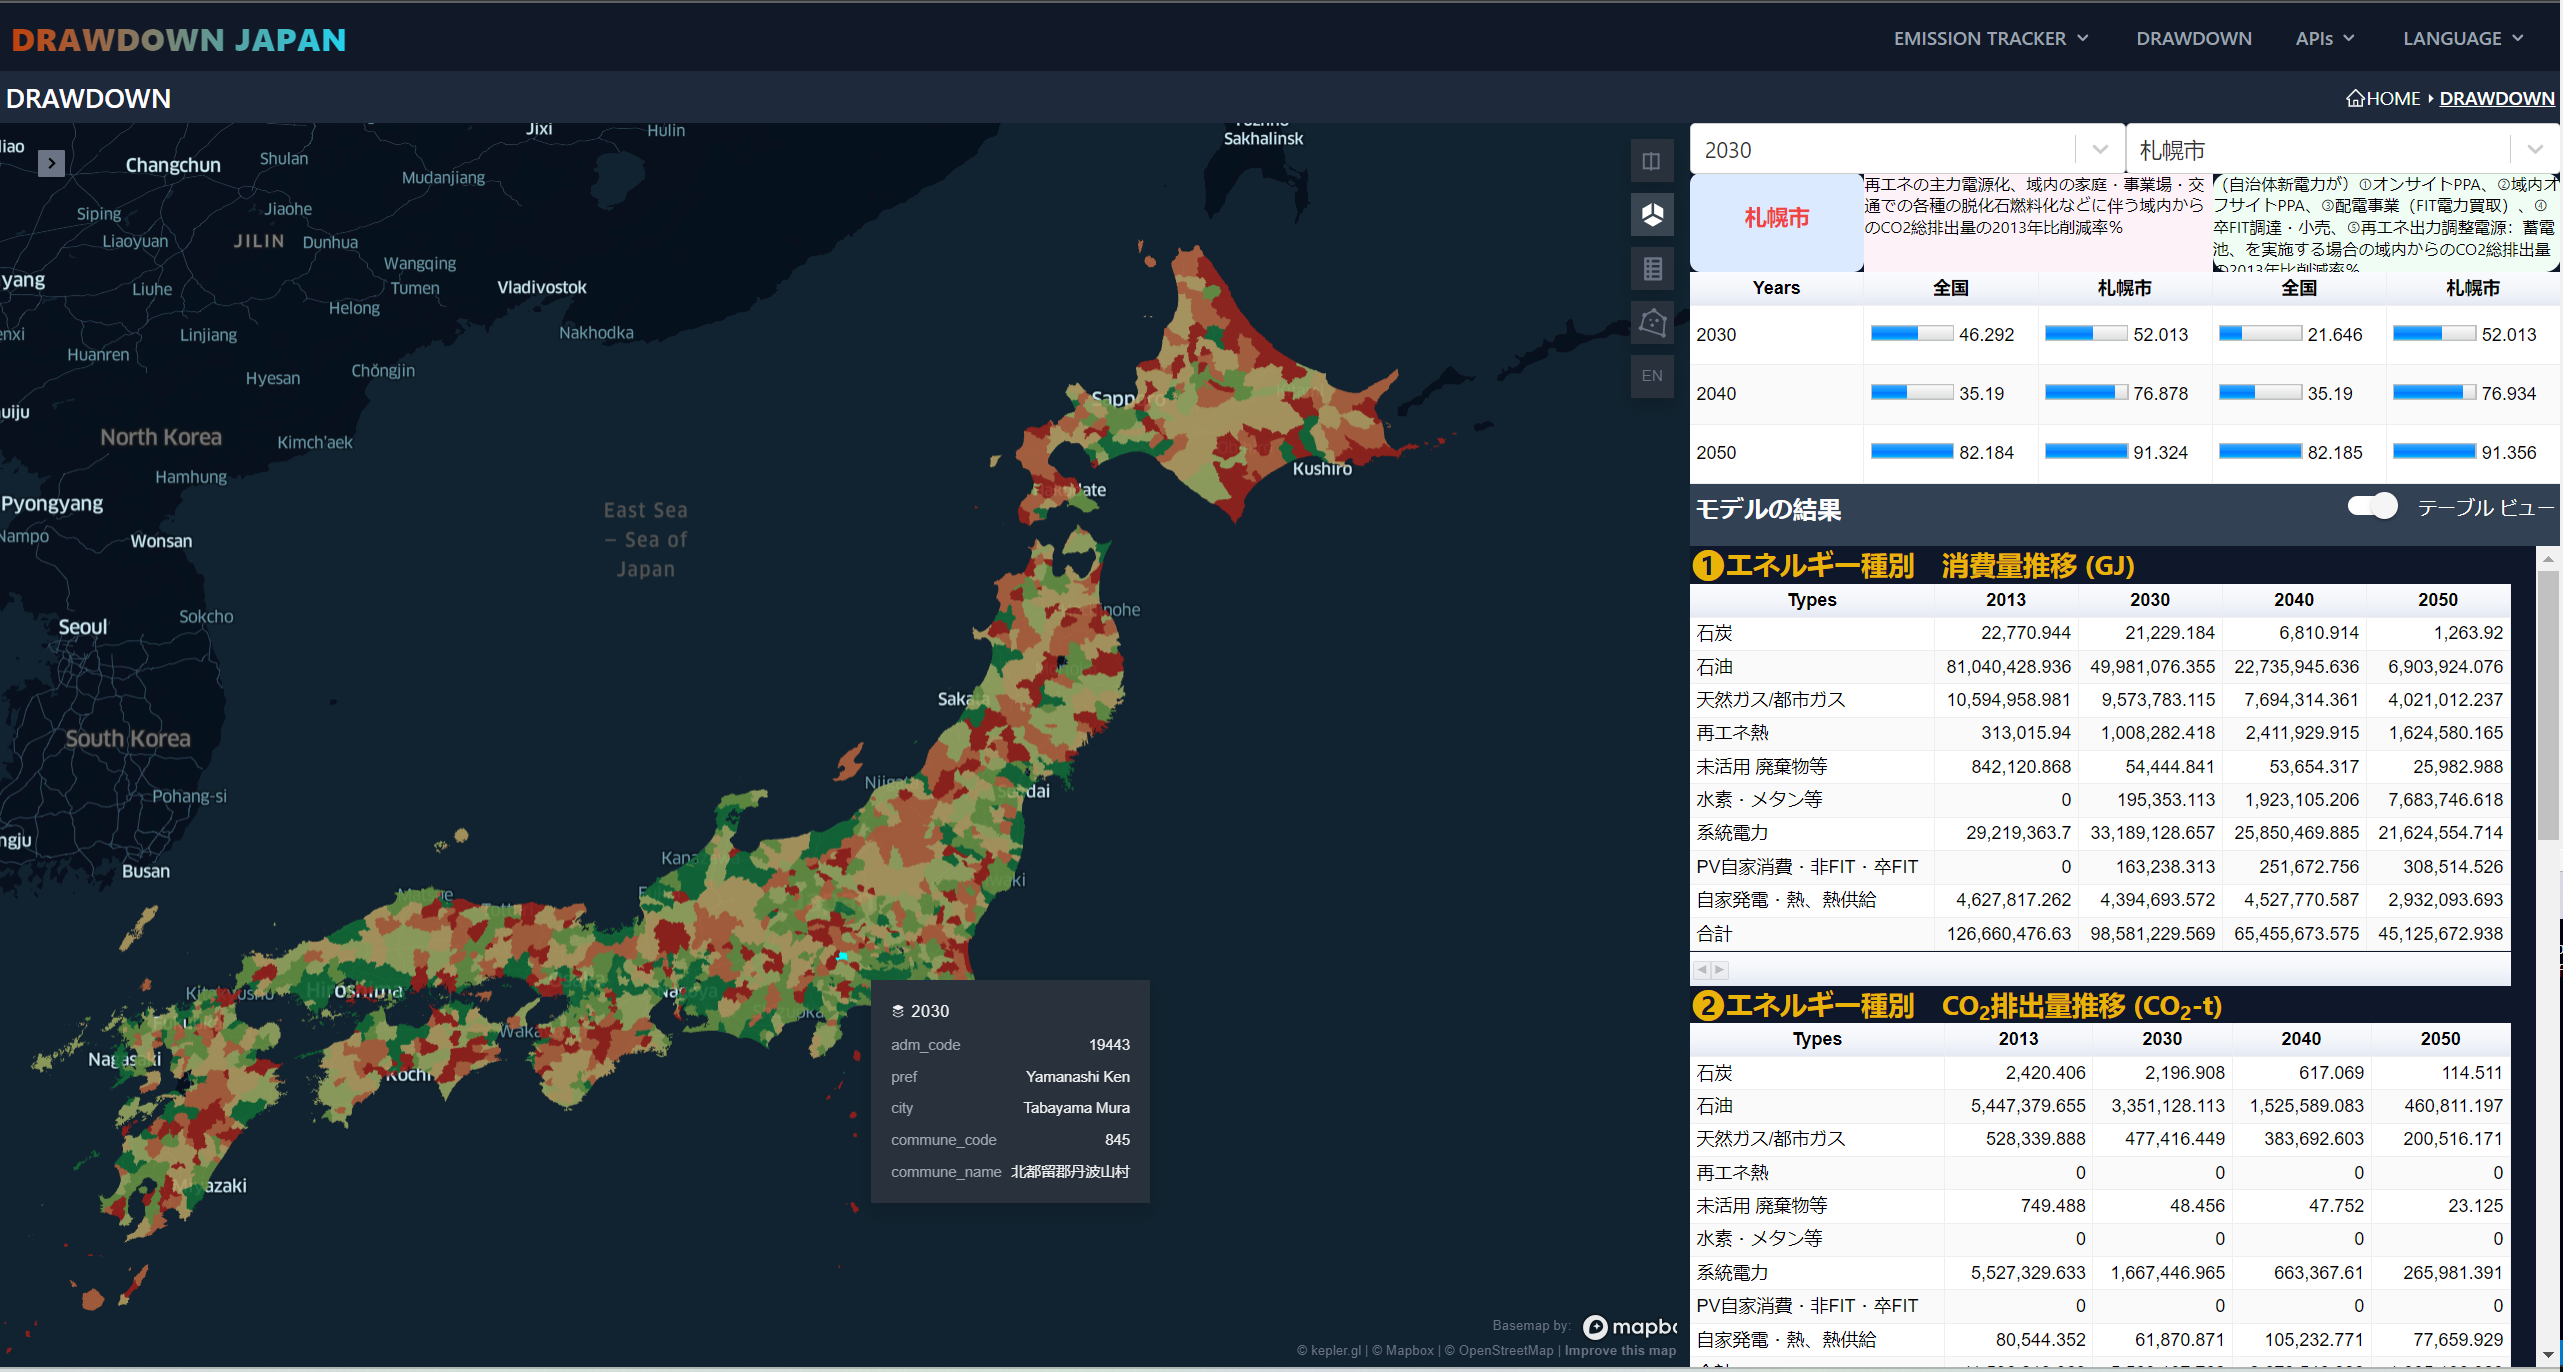
\includegraphics[width=.9\textwidth]{figs/chap7/drawdown2.png}
      \caption{Map overlays}
      % \label{fig:chap7_fig2b}
  \end{subfigure}
  \caption[Inferred forest map in Ena City]{Inferred forest map in Ena City, Japan \textminus 2018 (OA \textminus 94.5\%)}
  \label{fig:chap7_fig3}
\end{figure}

\begin{figure}[tbh!]
  \centering
  \begin{subfigure}{.5\textwidth}
      \centering
      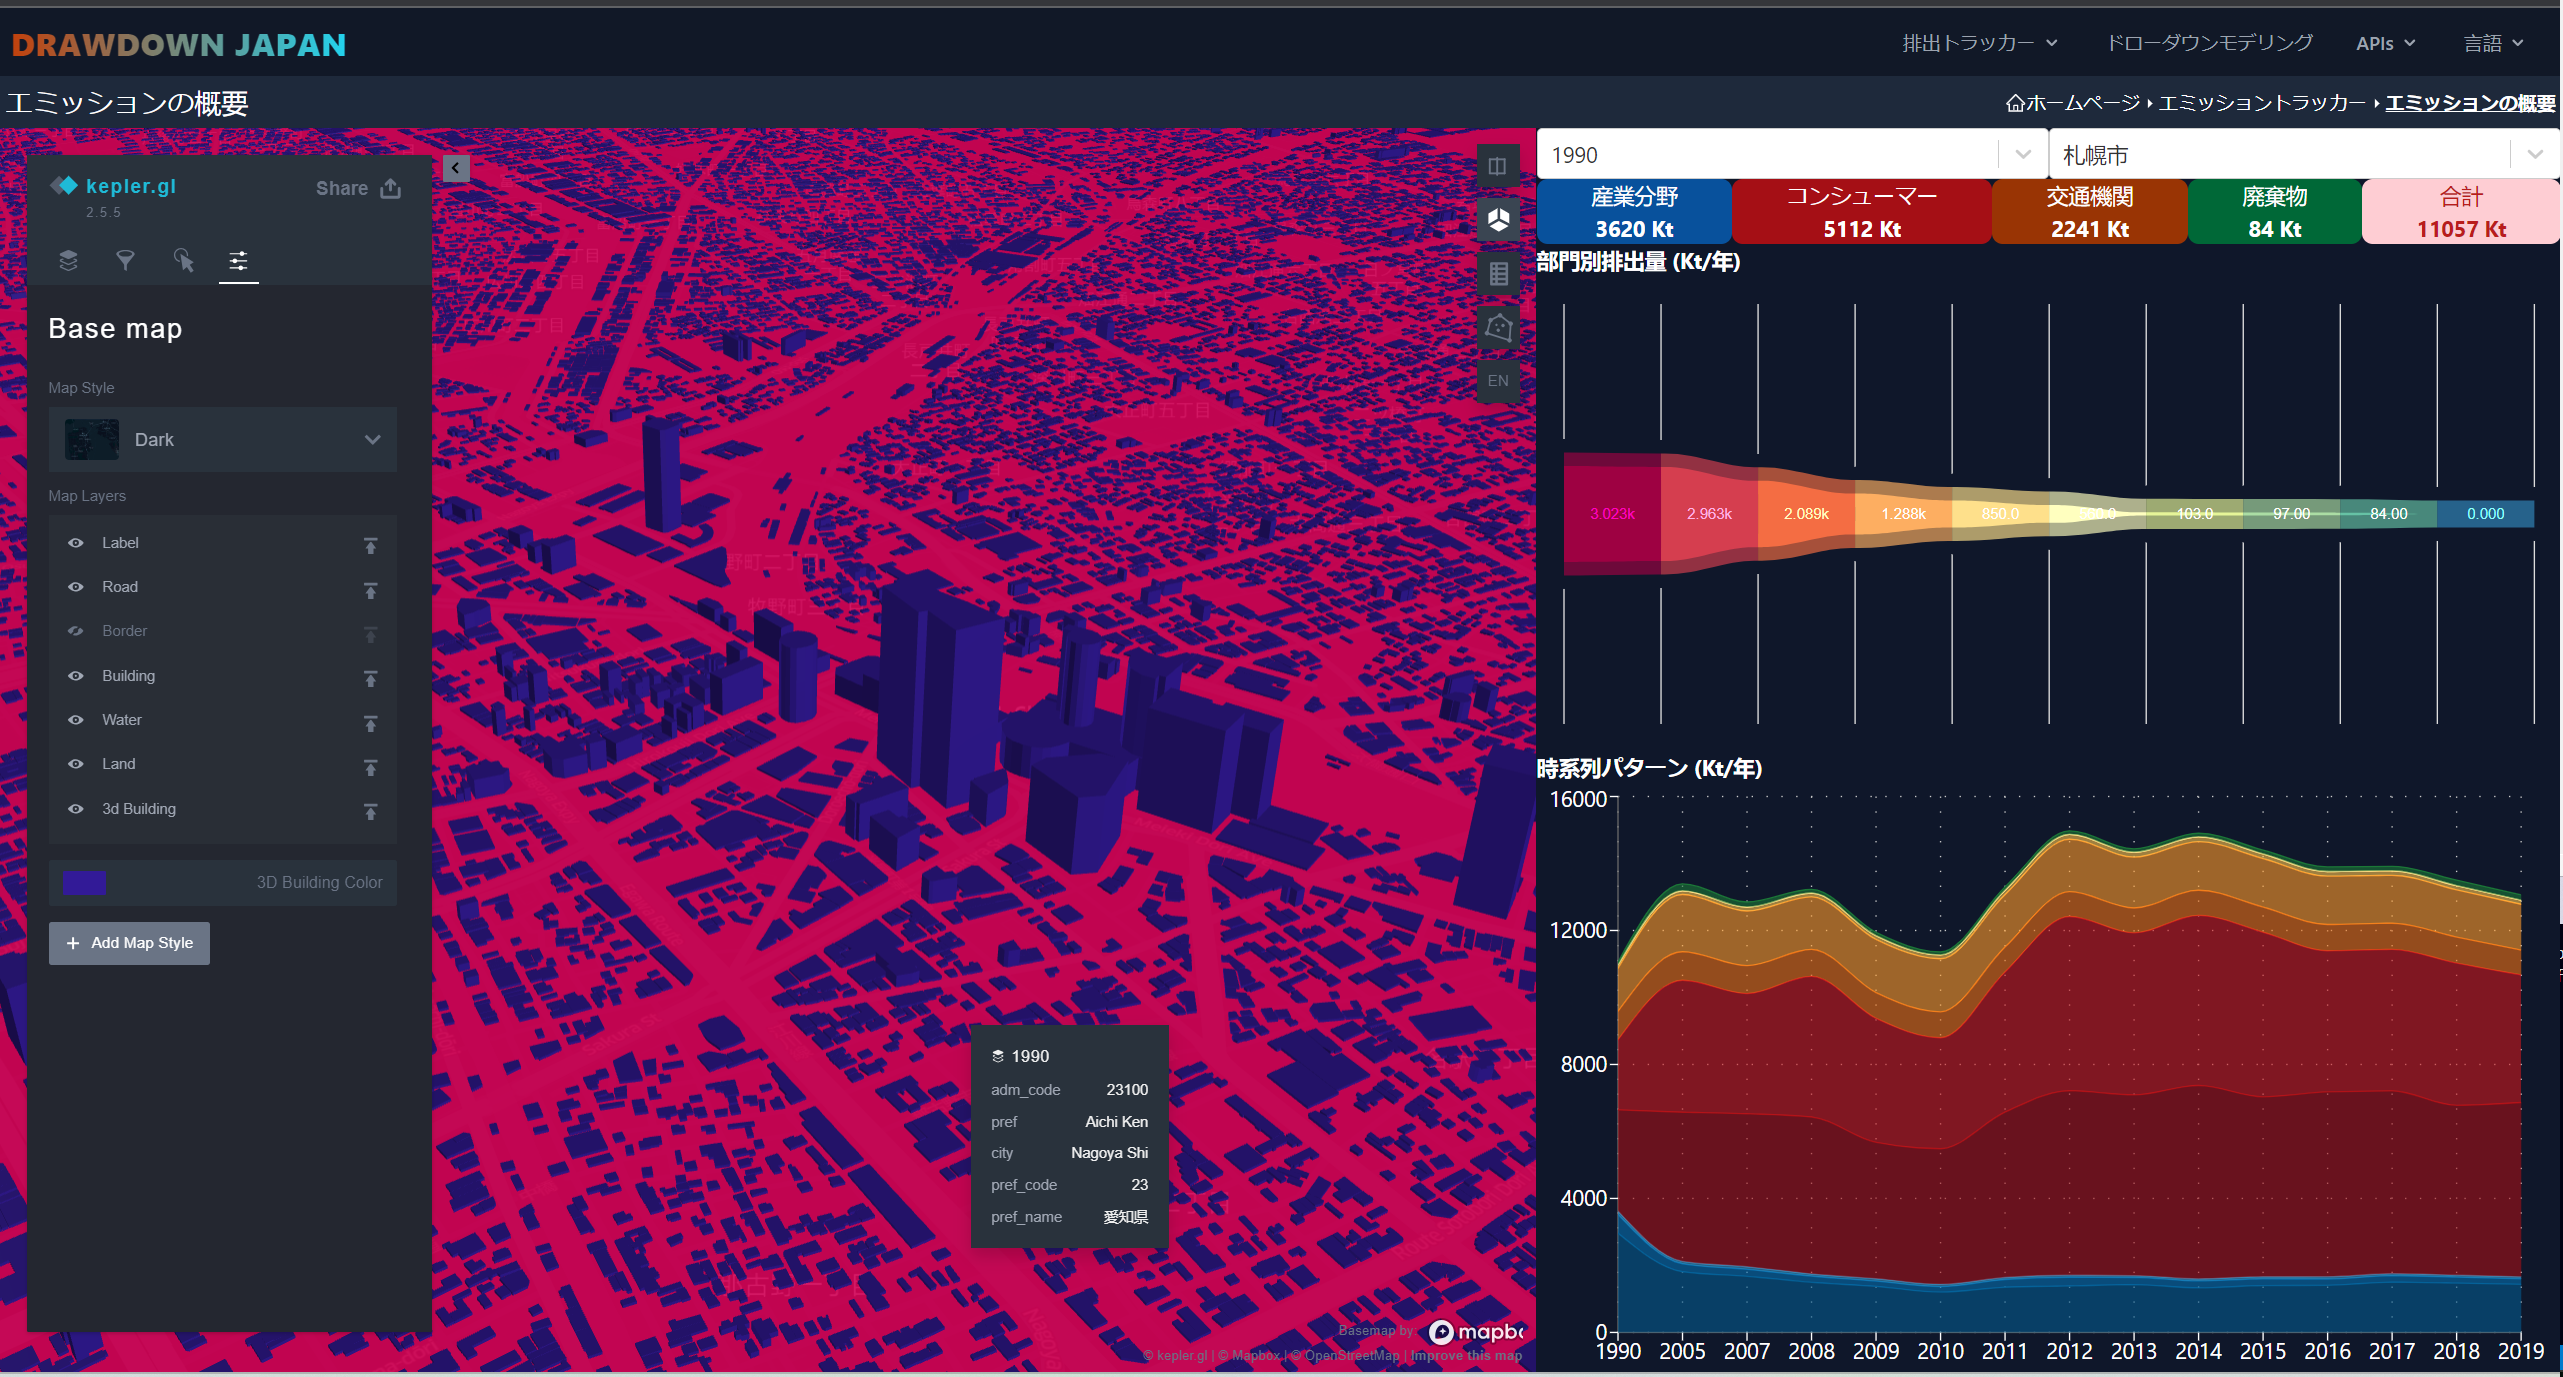
\includegraphics[width=.9\textwidth]{figs/chap7/3d_bldg.png}
      \caption{Forest map in Ena City, Japan}
      % \label{fig:chap7_fig2a}
  \end{subfigure}%
  \begin{subfigure}{.5\textwidth}
      \centering
      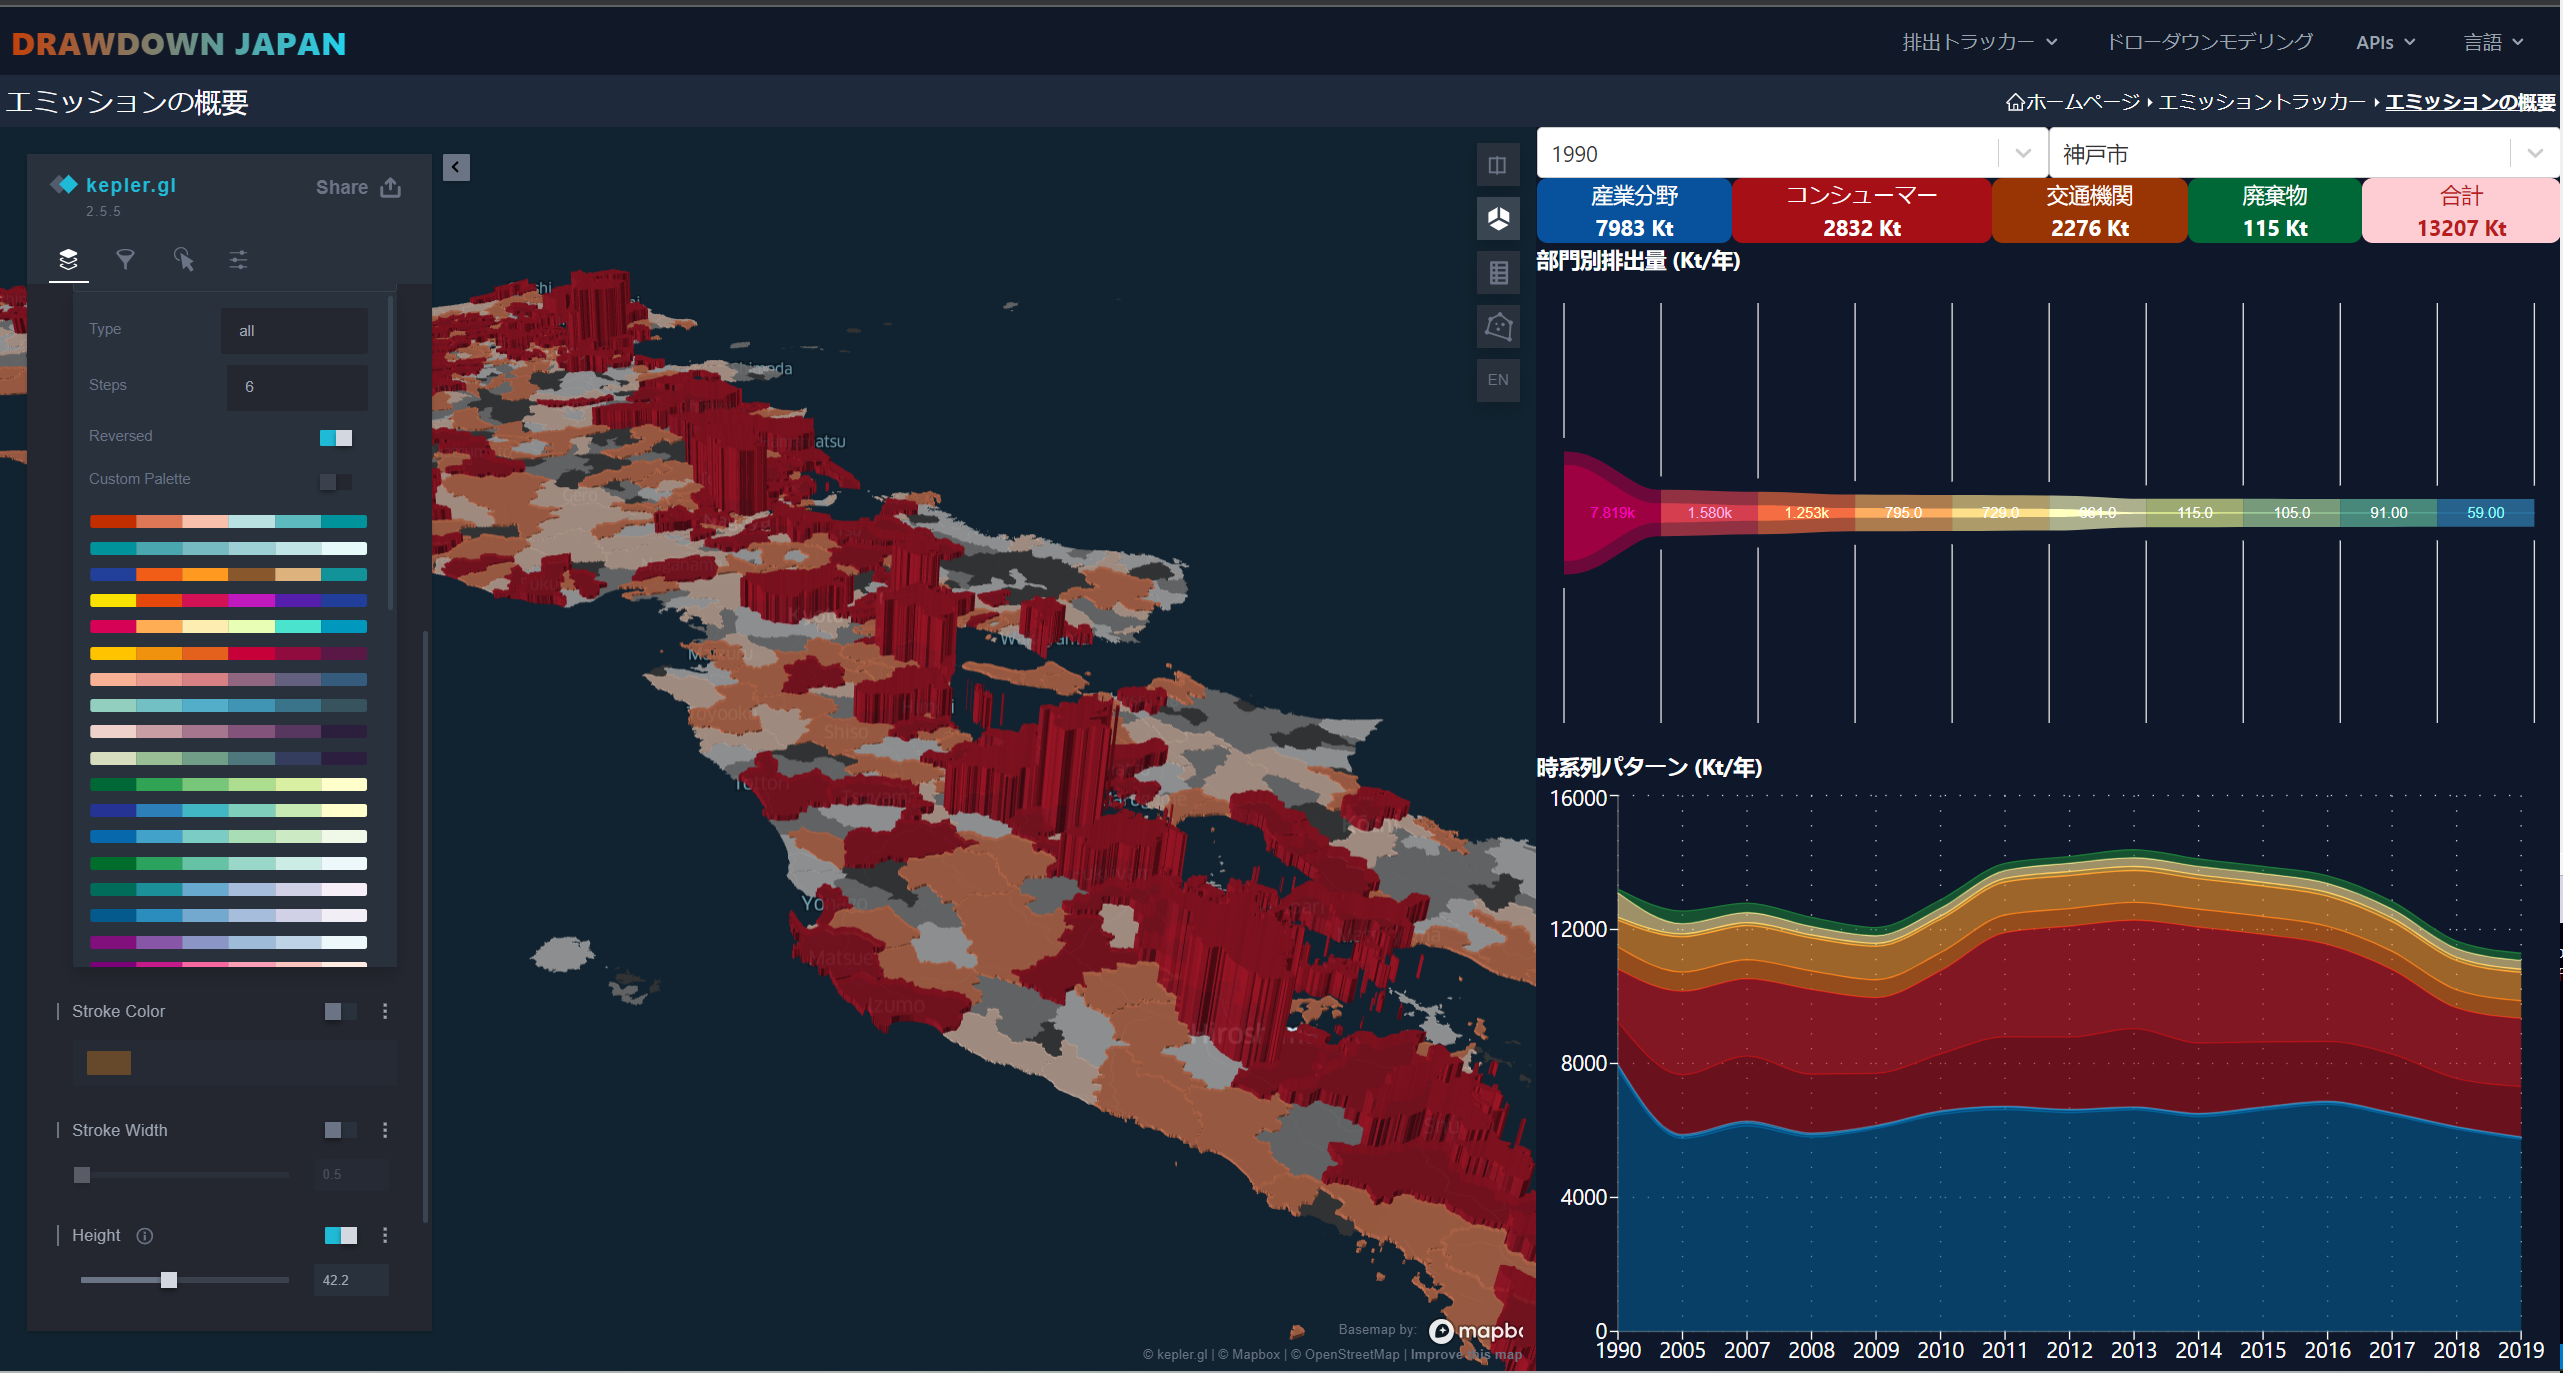
\includegraphics[width=.9\textwidth]{figs/chap7/3d_ja.png}
      \caption{Map overlays}
      % \label{fig:chap7_fig2b}
  \end{subfigure}
  \caption[Inferred forest map in Ena City]{Inferred forest map in Ena City, Japan \textminus 2018 (OA \textminus 94.5\%)}
  \label{fig:chap7_fig3}
\end{figure}

\begin{figure}[tbh!]
  \centering
  \begin{subfigure}{.5\textwidth}
      \centering
      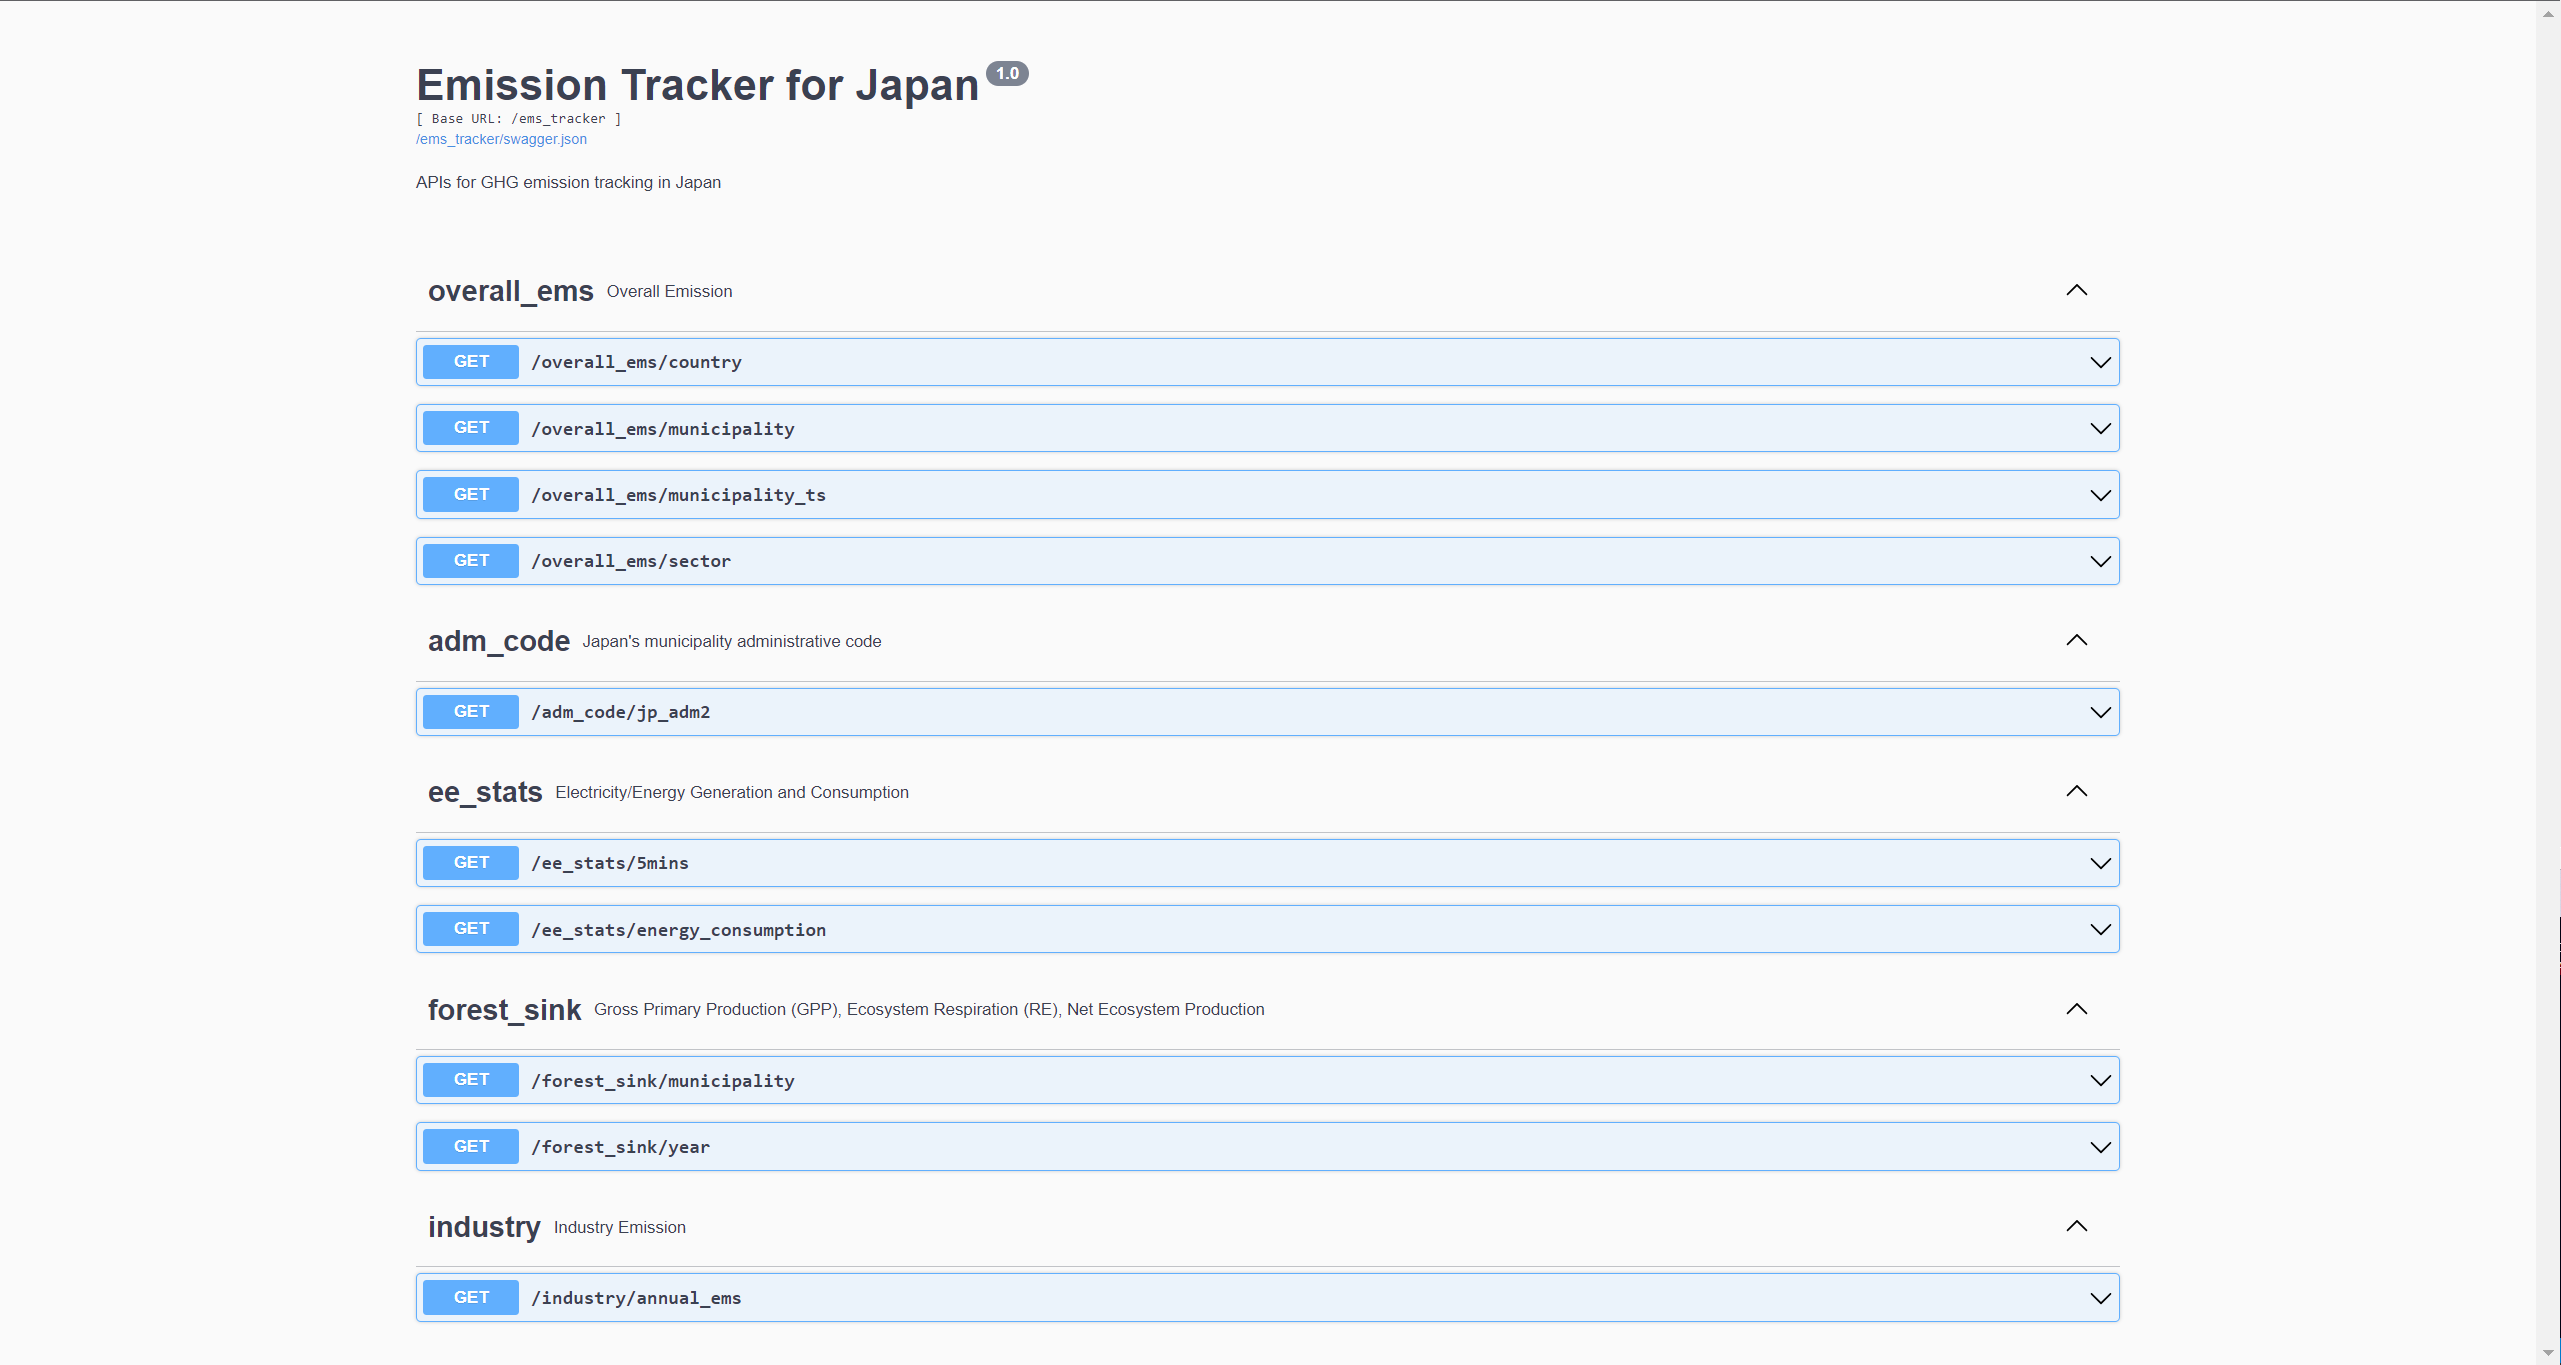
\includegraphics[width=.9\textwidth]{figs/chap7/api1.png}
      \caption{Forest map in Ena City, Japan}
      % \label{fig:chap7_fig2a}
  \end{subfigure}%
  \begin{subfigure}{.5\textwidth}
      \centering
      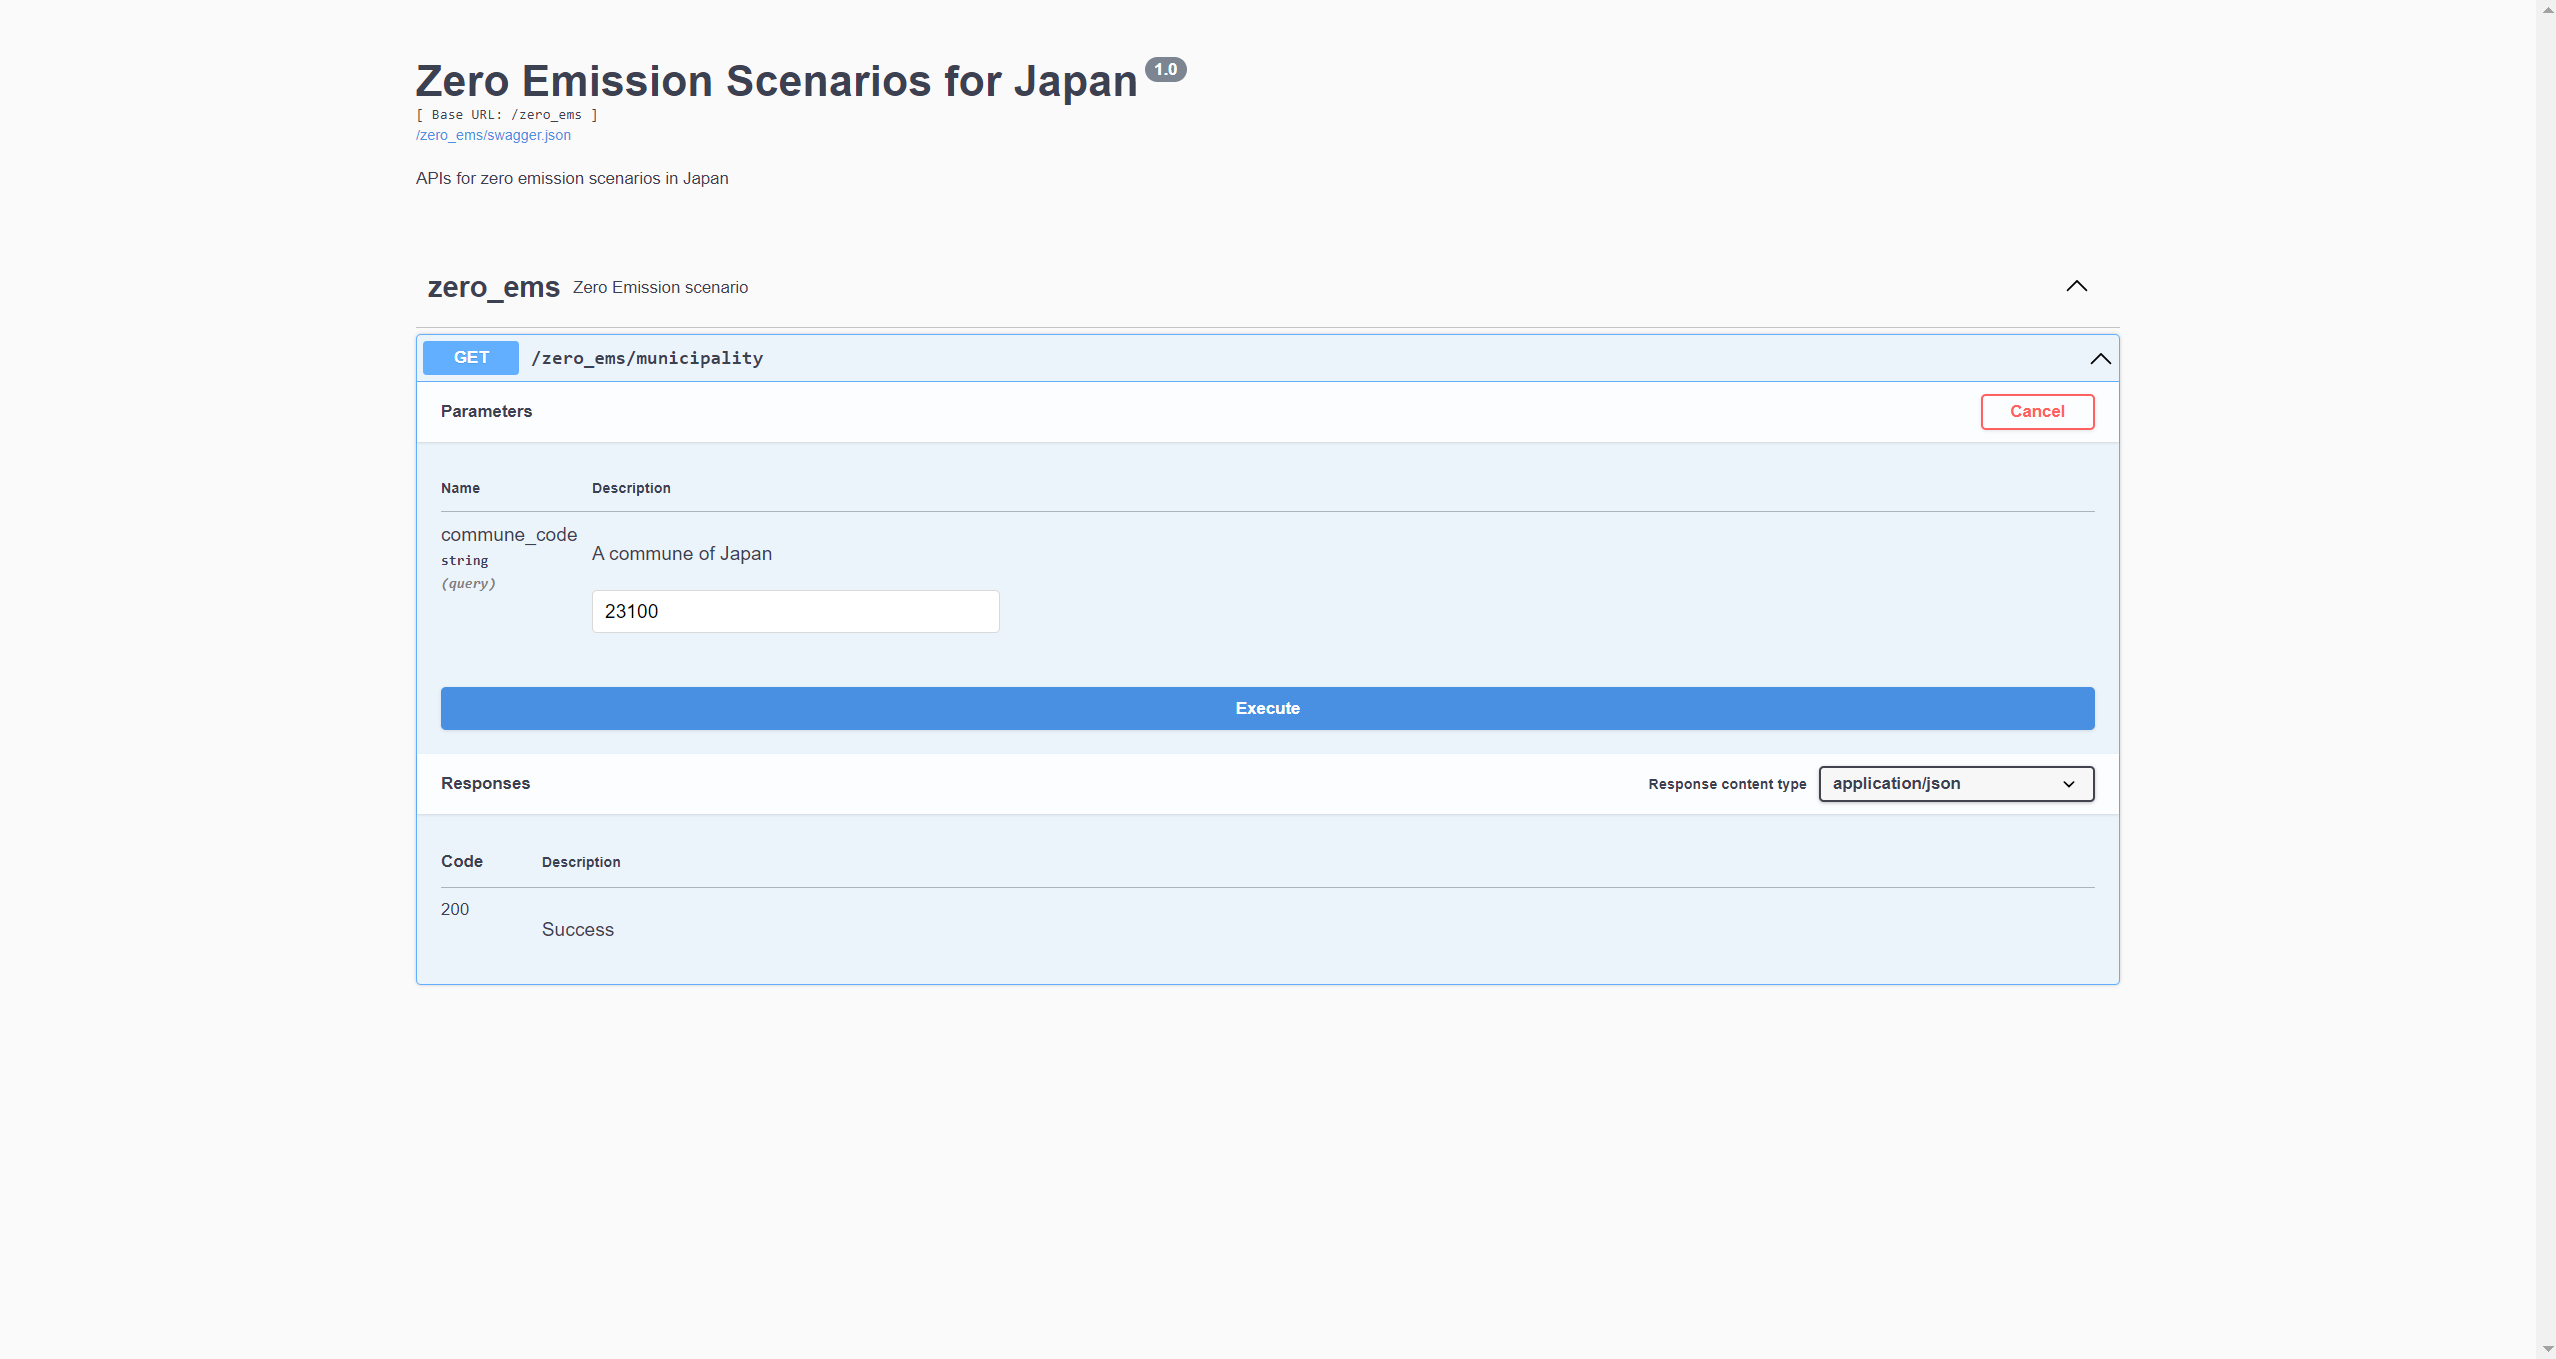
\includegraphics[width=.9\textwidth]{figs/chap7/api2.png}
      \caption{Map overlays}
      % \label{fig:chap7_fig2b}
  \end{subfigure}
  \caption[Inferred forest map in Ena City]{Inferred forest map in Ena City, Japan \textminus 2018 (OA \textminus 94.5\%)}
  \label{fig:chap7_fig3}
\end{figure}


\begin{itemize}
    \item Web Application: Node.js, ReactJS, Redux
    \item Interactive Charts: Rechart, React Google Charts, NIVO
    \item Interactive Maps: Mapbox and Kepler.gl
\end{itemize}
\section{Result and discussion}
\subsection{Result}
The overview of usage scenarios for the developed GIS platform is outlined below, along with the interface of the platform's main page (refer to Figure 2). The GIS platform conducts visualization using maps and charts.\par

The Emission Tracker provides information on emissions and energy consumption at the municipal level. Visualized data is organized into tabs, including an overview of emissions, energy consumption, electricity statistics, industrial emissions, and forest absorption. Users can start accessing relevant information by selecting a municipality of interest using a dropdown selection box or a map.\par

[Overview of Emissions]: This tab displays emission data classified by sector (industry, residential, transportation, waste) from 1990 to 2019. It provides an understanding of the current state and temporal changes in emissions.\par

[Energy Consumption]: This tab offers detailed information on energy consumption at the municipal level in Japan from 2013 to 2019. The data is aggregated by energy type and sector. It supports decision-making on efficient energy use and savings.\par

[Electricity Statistics]: This tab provides information on the spatial distribution of power plants in Japan, aggregated by plant type. It includes data from major domestic power companies on electricity usage, usage forecasts, and supply forecasts, obtained through web scraping technology.\par

[Industrial Emissions]: This tab offers a comprehensive view of industrial sector emissions, presenting emission profiles of each company (specific operators under the Energy Saving Act with a total energy usage of 1500kl/year or more) from 2009 to 2017. It uses reporting information based on the Energy Saving Act to aggregate municipal-level emissions and provides insights into the distribution of industrial emissions nationwide. It also ranks companies based on annual emissions within municipalities, offering reference information for monitoring industrial sector emissions.\par

[Forest Absorption]: This tab displays three key variables related to forest absorption: Gross Primary Production (GPP), Net Ecosystem Production (NEP), and ecosystem respiration. These variables, derived from simulations of the global model Vegetation Integrative Simulator for Trace Gas (VISIT), provide a long-term trend from 1901 to 2020. The data is visualized at the municipal level, presenting a rolling display of 5 years of data.\par

The "Drawdown" page introduces a comprehensive roadmap for reducing CO2 emissions by 2050 at the municipal level in Japan. Specifically, it presents a roadmap with various parameters, including trends in energy consumption, trends in CO2 emissions by energy type, trends in CO2 emissions by sector/industry, regional renewable energy electricity, regional production-consumption planning, and the ratio of total regional production-consumption to total energy usage. Additionally, it visualizes the total CO2 emissions reduction by 2030, 2040, and 2050. This allows municipal officials not only to understand their municipality's data in detail but also to deepen their understanding through personalized data comparisons with other similar municipalities using multi-screen comparisons. Figure 2 summarizes the interfaces corresponding to each function. While the Emission Tracker page is available in both English and Japanese, the Drawdown page is currently only available in Japanese. Moreover, API URLs are provided to allow users to access data programmatically and integrate it into their applications or software. This not only enhances the overall functionality of the platform in the future but also encourages knowledge sharing and the development of new applications to address the ongoing climate crisis. \par
The GIS platform is accessible at http://de14.digitalasia.chubu.ac.jp/.\par

\begin{lstlisting}[language=json,firstnumber=1][p]
  {
    "features": [
      {
        "geometry": {
          "coordinates": [
            [...]
          ],
          "type": "Polygon"
        },
        "id": "26",
        "properties": {
          "adm_code": 23100,
          "agriculture": 30,
          "building": 3435,
          "business": 5034,
          "city": "Nagoya Shi",
          "construction_mining": 235,
          "consumer_total": 8469,
          "freight_car": 1222,
          "industry_total": 3900,
          "manufacture": 3635,
          "passenger_car": 2134,
          "pref": "Aichi Ken",
          "pref_code": 23,
          "railway": 126,
          "ship": 46,
          "total": 16017,
          "transportation_total": 3528,
          "waste": 121
        },
        "type": "Feature"
      }
    ],
    "type": "FeatureCollection"
  }
\end{lstlisting}
\begin{lstlisting}[language=json,firstnumber=1][p]
  {
  "result": [
    {
      "agriculture": 39,
      "building": 2473,
      "business": 3032,
      "construction_mining": 311,
      "freight_car": 1478,
      "manufacture": 6910,
      "passenger_car": 1840,
      "railway": 133,
      "ship": 36,
      "waste": 144,
      "year": 1990
    },
    ...
    {
      "agriculture": 30,
      "building": 3435,
      "business": 5034,
      "construction_mining": 235,
      "freight_car": 1222,
      "manufacture": 3635,
      "passenger_car": 2134,
      "railway": 126,
      "ship": 46,
      "waste": 121,
      "year": 2005
    },
  ]
}
\end{lstlisting}


\subsection{Discussion}

When comparing this GIS platform to existing platforms like Project Drawdown [4] (refer to Figure 3a) and Drawdown Georgia [6] (refer to Figure 3b), the interface design may differ slightly, but the commonality lies in charts and maps being fundamental components.\par

The key distinction between this GIS platform and these existing platforms is that this platform has become an integrated Geo portal, utilizing GIS for all components from emission tracking to drawdown. This integration allows for a comprehensive representation of emission data and simultaneously provides a simulated roadmap, setting it apart from other platforms.\par
In the future, we plan to enhance the user interface based on user experience feedback and incorporate a global perspective into the system development.\par